\documentclass[journal]{IEEEtran}


\usepackage{times}
\usepackage{latexsym}

\usepackage[T1]{fontenc}

\usepackage[utf8]{inputenc}

\usepackage{microtype}

\usepackage{inconsolata}

\usepackage{graphicx}


\usepackage{amsmath}
\usepackage{amssymb}
\usepackage{multirow}
\usepackage{booktabs}
\usepackage{catchfile}

\usepackage[boxed]{algorithm}
\usepackage{varwidth}
\usepackage[noEnd=true,indLines=false]{algpseudocodex}
\usepackage{cleveref}
\makeatletter
\@addtoreset{ALG@line}{algorithm}
\renewcommand{\ALG@beginalgorithmic}{\small}
\algrenewcommand\alglinenumber[1]{\small #1:}
\makeatother

\usepackage[normalem]{ulem}
\usepackage{todonotes}

\usepackage{lipsum}    %
\usepackage{comment}   %
\usepackage{graphicx}  %
\usepackage{pifont}    %

\usepackage[font=small,labelfont=bf]{caption}
\usepackage{float}     %
\usepackage{booktabs}  %
\usepackage{subcaption}  %

\usepackage{listings}

\usepackage{amsthm}  %

\hyphenation{op-tical net-works semi-conduc-tor IEEE-Xplore}
\def\BibTeX{{\rm B\kern-.05em{\sc i\kern-.025em b}\kern-.08em
    T\kern-.1667em\lower.7ex\hbox{E}\kern-.125emX}}

\begin{document}

\title{\system: Automated Migration and Protection of Programs in Trusted Execution Environments}


\author{Ruidong Han~\textsuperscript{\orcidlink{0000-0001-6859-60057}},
        Zhou Yang~\textsuperscript{\orcidlink{0000-0001-5938-1918}},
        Chengyan Ma~\textsuperscript{\orcidlink{0000-0001-9256-6930}},
        Ye Liu~\textsuperscript{\orcidlink{0000-0003-4562-8208}},
        Yuqing Niu, \\
        Siqi Ma~\textsuperscript{\orcidlink{0000-0003-3479-5713}}, ~\IEEEmembership{Member,~IEEE}, 
        Debin Gao~\textsuperscript{\orcidlink{0000-0001-9412-9961}},~\IEEEmembership{Member,~IEEE},
        David Lo~\textsuperscript{\orcidlink{0000-0002-4367-7201}},~\IEEEmembership{Fellow,~IEEE}

\thanks{
Ruidong Han, Zhou Yang, Chengyan Ma, Ye Liu, Yuqing Niu, Debin Gao, and David Lo are with the School of Computing and Information Systems, Singapore Management University, Singapore (e-mail:rdhan@smu.edu.sg; zyang@smu.edu.sg, chengyanma@smu.edu.sg; yeliu@smu.edu.sg; yuqingniu@smu.edu.sg; dbgao@smu.edu.sg; davidlo@smu.edu.sg).
Siqi Ma is with the School of Computer Science and Engineering, UNSW Sydney, Australia (e-mail:siqi.ma@unsw.edu.au).
}

}

\markboth{Journal of \LaTeX\ Class Files,~Vol.~18, No.~9, September~2025}%
{\system: Automatically Protect Programs under Trusted Execution Environments}
	




\maketitle

\begin{abstract}
\begin{abstract}  
Test time scaling is currently one of the most active research areas that shows promise after training time scaling has reached its limits.
Deep-thinking (DT) models are a class of recurrent models that can perform easy-to-hard generalization by assigning more compute to harder test samples.
However, due to their inability to determine the complexity of a test sample, DT models have to use a large amount of computation for both easy and hard test samples.
Excessive test time computation is wasteful and can cause the ``overthinking'' problem where more test time computation leads to worse results.
In this paper, we introduce a test time training method for determining the optimal amount of computation needed for each sample during test time.
We also propose Conv-LiGRU, a novel recurrent architecture for efficient and robust visual reasoning. 
Extensive experiments demonstrate that Conv-LiGRU is more stable than DT, effectively mitigates the ``overthinking'' phenomenon, and achieves superior accuracy.
\end{abstract}  
\end{abstract}

%\IEEEpeerreviewmaketitle


\section{Introduction}
\label{sec:intro}
\section{Introduction}
\label{sec:introduction}
The business processes of organizations are experiencing ever-increasing complexity due to the large amount of data, high number of users, and high-tech devices involved \cite{martin2021pmopportunitieschallenges, beerepoot2023biggestbpmproblems}. This complexity may cause business processes to deviate from normal control flow due to unforeseen and disruptive anomalies \cite{adams2023proceddsriftdetection}. These control-flow anomalies manifest as unknown, skipped, and wrongly-ordered activities in the traces of event logs monitored from the execution of business processes \cite{ko2023adsystematicreview}. For the sake of clarity, let us consider an illustrative example of such anomalies. Figure \ref{FP_ANOMALIES} shows a so-called event log footprint, which captures the control flow relations of four activities of a hypothetical event log. In particular, this footprint captures the control-flow relations between activities \texttt{a}, \texttt{b}, \texttt{c} and \texttt{d}. These are the causal ($\rightarrow$) relation, concurrent ($\parallel$) relation, and other ($\#$) relations such as exclusivity or non-local dependency \cite{aalst2022pmhandbook}. In addition, on the right are six traces, of which five exhibit skipped, wrongly-ordered and unknown control-flow anomalies. For example, $\langle$\texttt{a b d}$\rangle$ has a skipped activity, which is \texttt{c}. Because of this skipped activity, the control-flow relation \texttt{b}$\,\#\,$\texttt{d} is violated, since \texttt{d} directly follows \texttt{b} in the anomalous trace.
\begin{figure}[!t]
\centering
\includegraphics[width=0.9\columnwidth]{images/FP_ANOMALIES.png}
\caption{An example event log footprint with six traces, of which five exhibit control-flow anomalies.}
\label{FP_ANOMALIES}
\end{figure}

\subsection{Control-flow anomaly detection}
Control-flow anomaly detection techniques aim to characterize the normal control flow from event logs and verify whether these deviations occur in new event logs \cite{ko2023adsystematicreview}. To develop control-flow anomaly detection techniques, \revision{process mining} has seen widespread adoption owing to process discovery and \revision{conformance checking}. On the one hand, process discovery is a set of algorithms that encode control-flow relations as a set of model elements and constraints according to a given modeling formalism \cite{aalst2022pmhandbook}; hereafter, we refer to the Petri net, a widespread modeling formalism. On the other hand, \revision{conformance checking} is an explainable set of algorithms that allows linking any deviations with the reference Petri net and providing the fitness measure, namely a measure of how much the Petri net fits the new event log \cite{aalst2022pmhandbook}. Many control-flow anomaly detection techniques based on \revision{conformance checking} (hereafter, \revision{conformance checking}-based techniques) use the fitness measure to determine whether an event log is anomalous \cite{bezerra2009pmad, bezerra2013adlogspais, myers2018icsadpm, pecchia2020applicationfailuresanalysispm}. 

The scientific literature also includes many \revision{conformance checking}-independent techniques for control-flow anomaly detection that combine specific types of trace encodings with machine/deep learning \cite{ko2023adsystematicreview, tavares2023pmtraceencoding}. Whereas these techniques are very effective, their explainability is challenging due to both the type of trace encoding employed and the machine/deep learning model used \cite{rawal2022trustworthyaiadvances,li2023explainablead}. Hence, in the following, we focus on the shortcomings of \revision{conformance checking}-based techniques to investigate whether it is possible to support the development of competitive control-flow anomaly detection techniques while maintaining the explainable nature of \revision{conformance checking}.
\begin{figure}[!t]
\centering
\includegraphics[width=\columnwidth]{images/HIGH_LEVEL_VIEW.png}
\caption{A high-level view of the proposed framework for combining \revision{process mining}-based feature extraction with dimensionality reduction for control-flow anomaly detection.}
\label{HIGH_LEVEL_VIEW}
\end{figure}

\subsection{Shortcomings of \revision{conformance checking}-based techniques}
Unfortunately, the detection effectiveness of \revision{conformance checking}-based techniques is affected by noisy data and low-quality Petri nets, which may be due to human errors in the modeling process or representational bias of process discovery algorithms \cite{bezerra2013adlogspais, pecchia2020applicationfailuresanalysispm, aalst2016pm}. Specifically, on the one hand, noisy data may introduce infrequent and deceptive control-flow relations that may result in inconsistent fitness measures, whereas, on the other hand, checking event logs against a low-quality Petri net could lead to an unreliable distribution of fitness measures. Nonetheless, such Petri nets can still be used as references to obtain insightful information for \revision{process mining}-based feature extraction, supporting the development of competitive and explainable \revision{conformance checking}-based techniques for control-flow anomaly detection despite the problems above. For example, a few works outline that token-based \revision{conformance checking} can be used for \revision{process mining}-based feature extraction to build tabular data and develop effective \revision{conformance checking}-based techniques for control-flow anomaly detection \cite{singh2022lapmsh, debenedictis2023dtadiiot}. However, to the best of our knowledge, the scientific literature lacks a structured proposal for \revision{process mining}-based feature extraction using the state-of-the-art \revision{conformance checking} variant, namely alignment-based \revision{conformance checking}.

\subsection{Contributions}
We propose a novel \revision{process mining}-based feature extraction approach with alignment-based \revision{conformance checking}. This variant aligns the deviating control flow with a reference Petri net; the resulting alignment can be inspected to extract additional statistics such as the number of times a given activity caused mismatches \cite{aalst2022pmhandbook}. We integrate this approach into a flexible and explainable framework for developing techniques for control-flow anomaly detection. The framework combines \revision{process mining}-based feature extraction and dimensionality reduction to handle high-dimensional feature sets, achieve detection effectiveness, and support explainability. Notably, in addition to our proposed \revision{process mining}-based feature extraction approach, the framework allows employing other approaches, enabling a fair comparison of multiple \revision{conformance checking}-based and \revision{conformance checking}-independent techniques for control-flow anomaly detection. Figure \ref{HIGH_LEVEL_VIEW} shows a high-level view of the framework. Business processes are monitored, and event logs obtained from the database of information systems. Subsequently, \revision{process mining}-based feature extraction is applied to these event logs and tabular data input to dimensionality reduction to identify control-flow anomalies. We apply several \revision{conformance checking}-based and \revision{conformance checking}-independent framework techniques to publicly available datasets, simulated data of a case study from railways, and real-world data of a case study from healthcare. We show that the framework techniques implementing our approach outperform the baseline \revision{conformance checking}-based techniques while maintaining the explainable nature of \revision{conformance checking}.

In summary, the contributions of this paper are as follows.
\begin{itemize}
    \item{
        A novel \revision{process mining}-based feature extraction approach to support the development of competitive and explainable \revision{conformance checking}-based techniques for control-flow anomaly detection.
    }
    \item{
        A flexible and explainable framework for developing techniques for control-flow anomaly detection using \revision{process mining}-based feature extraction and dimensionality reduction.
    }
    \item{
        Application to synthetic and real-world datasets of several \revision{conformance checking}-based and \revision{conformance checking}-independent framework techniques, evaluating their detection effectiveness and explainability.
    }
\end{itemize}

The rest of the paper is organized as follows.
\begin{itemize}
    \item Section \ref{sec:related_work} reviews the existing techniques for control-flow anomaly detection, categorizing them into \revision{conformance checking}-based and \revision{conformance checking}-independent techniques.
    \item Section \ref{sec:abccfe} provides the preliminaries of \revision{process mining} to establish the notation used throughout the paper, and delves into the details of the proposed \revision{process mining}-based feature extraction approach with alignment-based \revision{conformance checking}.
    \item Section \ref{sec:framework} describes the framework for developing \revision{conformance checking}-based and \revision{conformance checking}-independent techniques for control-flow anomaly detection that combine \revision{process mining}-based feature extraction and dimensionality reduction.
    \item Section \ref{sec:evaluation} presents the experiments conducted with multiple framework and baseline techniques using data from publicly available datasets and case studies.
    \item Section \ref{sec:conclusions} draws the conclusions and presents future work.
\end{itemize}


\section{Background and Motivition}
\label{sec:back}
\section{Background}\label{sec:backgrnd}

\subsection{Cold Start Latency and Mitigation Techniques}

Traditional FaaS platforms mitigate cold starts through snapshotting, lightweight virtualization, and warm-state management. Snapshot-based methods like \textbf{REAP} and \textbf{Catalyzer} reduce initialization time by preloading or restoring container states but require significant memory and I/O resources, limiting scalability~\cite{dong_catalyzer_2020, ustiugov_benchmarking_2021}. Lightweight virtualization solutions, such as \textbf{Firecracker} microVMs, achieve fast startup times with strong isolation but depend on robust infrastructure, making them less adaptable to fluctuating workloads~\cite{agache_firecracker_2020}. Warm-state management techniques like \textbf{Faa\$T}~\cite{romero_faa_2021} and \textbf{Kraken}~\cite{vivek_kraken_2021} keep frequently invoked containers ready, balancing readiness and cost efficiency under predictable workloads but incurring overhead when demand is erratic~\cite{romero_faa_2021, vivek_kraken_2021}. While these methods perform well in resource-rich cloud environments, their resource intensity challenges applicability in edge settings.

\subsubsection{Edge FaaS Perspective}

In edge environments, cold start mitigation emphasizes lightweight designs, resource sharing, and hybrid task distribution. Lightweight execution environments like unikernels~\cite{edward_sock_2018} and \textbf{Firecracker}~\cite{agache_firecracker_2020}, as used by \textbf{TinyFaaS}~\cite{pfandzelter_tinyfaas_2020}, minimize resource usage and initialization delays but require careful orchestration to avoid resource contention. Function co-location, demonstrated by \textbf{Photons}~\cite{v_dukic_photons_2020}, reduces redundant initializations by sharing runtime resources among related functions, though this complicates isolation in multi-tenant setups~\cite{v_dukic_photons_2020}. Hybrid offloading frameworks like \textbf{GeoFaaS}~\cite{malekabbasi_geofaas_2024} balance edge-cloud workloads by offloading latency-tolerant tasks to the cloud and reserving edge resources for real-time operations, requiring reliable connectivity and efficient task management. These edge-specific strategies address cold starts effectively but introduce challenges in scalability and orchestration.

\subsection{Predictive Scaling and Caching Techniques}

Efficient resource allocation is vital for maintaining low latency and high availability in serverless platforms. Predictive scaling and caching techniques dynamically provision resources and reduce cold start latency by leveraging workload prediction and state retention.
Traditional FaaS platforms use predictive scaling and caching to optimize resources, employing techniques (OFC, FaasCache) to reduce cold starts. However, these methods rely on centralized orchestration and workload predictability, limiting their effectiveness in dynamic, resource-constrained edge environments.



\subsubsection{Edge FaaS Perspective}

Edge FaaS platforms adapt predictive scaling and caching techniques to constrain resources and heterogeneous environments. \textbf{EDGE-Cache}~\cite{kim_delay-aware_2022} uses traffic profiling to selectively retain high-priority functions, reducing memory overhead while maintaining readiness for frequent requests. Hybrid frameworks like \textbf{GeoFaaS}~\cite{malekabbasi_geofaas_2024} implement distributed caching to balance resources between edge and cloud nodes, enabling low-latency processing for critical tasks while offloading less critical workloads. Machine learning methods, such as clustering-based workload predictors~\cite{gao_machine_2020} and GRU-based models~\cite{guo_applying_2018}, enhance resource provisioning in edge systems by efficiently forecasting workload spikes. These innovations effectively address cold start challenges in edge environments, though their dependency on accurate predictions and robust orchestration poses scalability challenges.

\subsection{Decentralized Orchestration, Function Placement, and Scheduling}

Efficient orchestration in serverless platforms involves workload distribution, resource optimization, and performance assurance. While traditional FaaS platforms rely on centralized control, edge environments require decentralized and adaptive strategies to address unique challenges such as resource constraints and heterogeneous hardware.



\subsubsection{Edge FaaS Perspective}

Edge FaaS platforms adopt decentralized and adaptive orchestration frameworks to meet the demands of resource-constrained environments. Systems like \textbf{Wukong} distribute scheduling across edge nodes, enhancing data locality and scalability while reducing network latency. Lightweight frameworks such as \textbf{OpenWhisk Lite}~\cite{kravchenko_kpavelopenwhisk-light_2024} optimize resource allocation by decentralizing scheduling policies, minimizing cold starts and latency in edge setups~\cite{benjamin_wukong_2020}. Hybrid solutions like \textbf{OpenFaaS}~\cite{noauthor_openfaasfaas_2024} and \textbf{EdgeMatrix}~\cite{shen_edgematrix_2023} combine edge-cloud orchestration to balance resource utilization, retaining latency-sensitive functions at the edge while offloading non-critical workloads to the cloud. While these approaches improve flexibility, they face challenges in maintaining coordination and ensuring consistent performance across distributed nodes.



% \section{\system Overview}
% \label{sec:overview}
% \section{Overview}

\revision{In this section, we first explain the foundational concept of Hausdorff distance-based penetration depth algorithms, which are essential for understanding our method (Sec.~\ref{sec:preliminary}).
We then provide a brief overview of our proposed RT-based penetration depth algorithm (Sec.~\ref{subsec:algo_overview}).}



\section{Preliminaries }
\label{sec:Preliminaries}

% Before we introduce our method, we first overview the important basics of 3D dynamic human modeling with Gaussian splatting. Then, we discuss the diffusion-based 3d generation techniques, and how they can be applied to human modeling.
% \ZY{I stopp here. TBC.}
% \subsection{Dynamic human modeling with Gaussian splatting}
\subsection{3D Gaussian Splatting}
3D Gaussian splatting~\cite{kerbl3Dgaussians} is an explicit scene representation that allows high-quality real-time rendering. The given scene is represented by a set of static 3D Gaussians, which are parameterized as follows: Gaussian center $x\in {\mathbb{R}^3}$, color $c\in {\mathbb{R}^3}$, opacity $\alpha\in {\mathbb{R}}$, spatial rotation in the form of quaternion $q\in {\mathbb{R}^4}$, and scaling factor $s\in {\mathbb{R}^3}$. Given these properties, the rendering process is represented as:
\begin{equation}
  I = Splatting(x, c, s, \alpha, q, r),
  \label{eq:splattingGA}
\end{equation}
where $I$ is the rendered image, $r$ is a set of query rays crossing the scene, and $Splatting(\cdot)$ is a differentiable rendering process. We refer readers to Kerbl et al.'s paper~\cite{kerbl3Dgaussians} for the details of Gaussian splatting. 



% \ZY{I would suggest move this part to the method part.}
% GaissianAvatar is a dynamic human generation model based on Gaussian splitting. Given a sequence of RGB images, this method utilizes fitted SMPLs and sampled points on its surface to obtain a pose-dependent feature map by a pose encoder. The pose-dependent features and a geometry feature are fed in a Gaussian decoder, which is employed to establish a functional mapping from the underlying geometry of the human form to diverse attributes of 3D Gaussians on the canonical surfaces. The parameter prediction process is articulated as follows:
% \begin{equation}
%   (\Delta x,c,s)=G_{\theta}(S+P),
%   \label{eq:gaussiandecoder}
% \end{equation}
%  where $G_{\theta}$ represents the Gaussian decoder, and $(S+P)$ is the multiplication of geometry feature S and pose feature P. Instead of optimizing all attributes of Gaussian, this decoder predicts 3D positional offset $\Delta{x} \in {\mathbb{R}^3}$, color $c\in\mathbb{R}^3$, and 3D scaling factor $ s\in\mathbb{R}^3$. To enhance geometry reconstruction accuracy, the opacity $\alpha$ and 3D rotation $q$ are set to fixed values of $1$ and $(1,0,0,0)$ respectively.
 
%  To render the canonical avatar in observation space, we seamlessly combine the Linear Blend Skinning function with the Gaussian Splatting~\cite{kerbl3Dgaussians} rendering process: 
% \begin{equation}
%   I_{\theta}=Splatting(x_o,Q,d),
%   \label{eq:splatting}
% \end{equation}
% \begin{equation}
%   x_o = T_{lbs}(x_c,p,w),
%   \label{eq:LBS}
% \end{equation}
% where $I_{\theta}$ represents the final rendered image, and the canonical Gaussian position $x_c$ is the sum of the initial position $x$ and the predicted offset $\Delta x$. The LBS function $T_{lbs}$ applies the SMPL skeleton pose $p$ and blending weights $w$ to deform $x_c$ into observation space as $x_o$. $Q$ denotes the remaining attributes of the Gaussians. With the rendering process, they can now reposition these canonical 3D Gaussians into the observation space.



\subsection{Score Distillation Sampling}
Score Distillation Sampling (SDS)~\cite{poole2022dreamfusion} builds a bridge between diffusion models and 3D representations. In SDS, the noised input is denoised in one time-step, and the difference between added noise and predicted noise is considered SDS loss, expressed as:

% \begin{equation}
%   \mathcal{L}_{SDS}(I_{\Phi}) \triangleq E_{t,\epsilon}[w(t)(\epsilon_{\phi}(z_t,y,t)-\epsilon)\frac{\partial I_{\Phi}}{\partial\Phi}],
%   \label{eq:SDSObserv}
% \end{equation}
\begin{equation}
    \mathcal{L}_{\text{SDS}}(I_{\Phi}) \triangleq \mathbb{E}_{t,\epsilon} \left[ w(t) \left( \epsilon_{\phi}(z_t, y, t) - \epsilon \right) \frac{\partial I_{\Phi}}{\partial \Phi} \right],
  \label{eq:SDSObservGA}
\end{equation}
where the input $I_{\Phi}$ represents a rendered image from a 3D representation, such as 3D Gaussians, with optimizable parameters $\Phi$. $\epsilon_{\phi}$ corresponds to the predicted noise of diffusion networks, which is produced by incorporating the noise image $z_t$ as input and conditioning it with a text or image $y$ at timestep $t$. The noise image $z_t$ is derived by introducing noise $\epsilon$ into $I_{\Phi}$ at timestep $t$. The loss is weighted by the diffusion scheduler $w(t)$. 
% \vspace{-3mm}

\subsection{Overview of the RTPD Algorithm}\label{subsec:algo_overview}
Fig.~\ref{fig:Overview} presents an overview of our RTPD algorithm.
It is grounded in the Hausdorff distance-based penetration depth calculation method (Sec.~\ref{sec:preliminary}).
%, similar to that of Tang et al.~\shortcite{SIG09HIST}.
The process consists of two primary phases: penetration surface extraction and Hausdorff distance calculation.
We leverage the RTX platform's capabilities to accelerate both of these steps.

\begin{figure*}[t]
    \centering
    \includegraphics[width=0.8\textwidth]{Image/overview.pdf}
    \caption{The overview of RT-based penetration depth calculation algorithm overview}
    \label{fig:Overview}
\end{figure*}

The penetration surface extraction phase focuses on identifying the overlapped region between two objects.
\revision{The penetration surface is defined as a set of polygons from one object, where at least one of its vertices lies within the other object. 
Note that in our work, we focus on triangles rather than general polygons, as they are processed most efficiently on the RTX platform.}
To facilitate this extraction, we introduce a ray-tracing-based \revision{Point-in-Polyhedron} test (RT-PIP), significantly accelerated through the use of RT cores (Sec.~\ref{sec:RT-PIP}).
This test capitalizes on the ray-surface intersection capabilities of the RTX platform.
%
Initially, a Geometry Acceleration Structure (GAS) is generated for each object, as required by the RTX platform.
The RT-PIP module takes the GAS of one object (e.g., $GAS_{A}$) and the point set of the other object (e.g., $P_{B}$).
It outputs a set of points (e.g., $P_{\partial B}$) representing the penetration region, indicating their location inside the opposing object.
Subsequently, a penetration surface (e.g., $\partial B$) is constructed using this point set (e.g., $P_{\partial B}$) (Sec.~\ref{subsec:surfaceGen}).
%
The generated penetration surfaces (e.g., $\partial A$ and $\partial B$) are then forwarded to the next step. 

The Hausdorff distance calculation phase utilizes the ray-surface intersection test of the RTX platform (Sec.~\ref{sec:RT-Hausdorff}) to compute the Hausdorff distance between two objects.
We introduce a novel Ray-Tracing-based Hausdorff DISTance algorithm, RT-HDIST.
It begins by generating GAS for the two penetration surfaces, $P_{\partial A}$ and $P_{\partial B}$, derived from the preceding step.
RT-HDIST processes the GAS of a penetration surface (e.g., $GAS_{\partial A}$) alongside the point set of the other penetration surface (e.g., $P_{\partial B}$) to compute the penetration depth between them.
The algorithm operates bidirectionally, considering both directions ($\partial A \to \partial B$ and $\partial B \to \partial A$).
The final penetration depth between the two objects, A and B, is determined by selecting the larger value from these two directional computations.

%In the Hausdorff distance calculation step, we compute the Hausdorff distance between given two objects using a ray-surface-intersection test. (Sec.~\ref{sec:RT-Hausdorff}) Initially, we construct the GAS for both $\partial A$ and $\partial B$ to utilize the RT-core effectively. The RT-based Hausdorff distance algorithms then determine the Hausdorff distance by processing the GAS of one object (e.g. $GAS_{\partial A}$) and set of the vertices of the other (e.g. $P_{\partial B}$). Following the Hausdorff distance definition (Eq.~\ref{equation:hausdorff_definition}), we compute the Hausdorff distance to both directions ($\partial A \to \partial B$) and ($\partial B \to \partial A$). As a result, the bigger one is the final Hausdorff distance, and also it is the penetration depth between input object $A$ and $B$.


%the proposed RT-based penetration depth calculation pipeline.
%Our proposed methods adopt Tang's Hausdorff-based penetration depth methods~\cite{SIG09HIST}. The pipeline is divided into the penetration surface extraction step and the Hausdorff distance calculation between the penetration surface steps. However, since Tang's approach is not suitable for the RT platform in detail, we modified and applied it with appropriate methods.

%The penetration surface extraction step is extracting overlapped surfaces on other objects. To utilize the RT core, we use the ray-intersection-based PIP(Point-In-Polygon) algorithms instead of collision detection between two objects which Tang et al.~\cite{SIG09HIST} used. (Sec.~\ref{sec:RT-PIP})
%RT core-based PIP test uses a ray-surface intersection test. For purpose this, we generate the GAS(Geometry Acceleration Structure) for each object. RT core-based PIP test takes the GAS of one object (e.g. $GAS_{A}$) and a set of vertex of another one (e.g. $P_{B}$). Then this computes the penetrated vertex set of another one (e.g. $P_{\partial B}$). To calculate the Hausdorff distance, these vertex sets change to objects constructed by penetrated surface (e.g. $\partial B$). Finally, the two generated overlapped surface objects $\partial A$ and $\partial B$ are used in the Hausdorff distance calculation step.

\section{\system}
\label{sec:design}
\section{The \search\ Search Algorithm}
\label{sec:search}

%In traditional ML, structure changes and step (operator) changes are performed before model training, \ie, fixed to the training process, and weights are updated with SGD, because weights are continous, differentiable values, and there are significantly more weights than structure and operator changes. In workflow autotuning, all three types of cogs can be chosen with a unified search-based approach, because all of them are non-differentiable configurations and the number of cogs in different types are all small.
%Thus, \sysname\ only needs to navigate the search space of combination of cogs as the search space to produce its workflow optimization results.

%We propose, \textit{\textbf{\search}}, an adaptive hierarchical search algorithm that autotunes gen-AI workflows based on observed end-to-end workflow results. In each search iteration, \search\ selects a combination of cogs to apply to the workflow and executes the resulting workflow with user-provided training inputs. \search\ evaluates the final generation quality using the user-specified evaluator and measures the execution time and cost for each training input. These results are aggregated and serve as BO observations and pruning criteria.
%the optimizer can condition on and propose better configurations in later trials. The optimizer will also be informed about the violation of any user-specified metric thresholds. More details of this mechanism can be found in Appendix ~\ref{appdx:TPE}.

With our insights in Section~\ref{sec:theory}, we believe that search methods based on Bayesian Optimizer (BO) can work for all types of cogs in gen-AI workflow autotuning because of BO's efficiency in searching discrete search space.
A key challenge in designing a BO-based search is the limited search budgets that need to be used to search a high-dimensional cog space. 
For example, for 4 cogs each with 4 options and a workflow of 3 LLM steps, the search space is $4^{12}$. Suppose each search uses GPT-4o and has 1000 output tokens, the entire space needs around \$168K to go through. A user search budget of \$100 can cover only 0.06\% of the search space. A traditional BO approach cannot find good results with such small budgets.
%The entire search space grows exponentially with the number of cogs and the number of steps in a workflow. Moreover, different cogs and different combinations of cogs can have varying impacts on different workflows. 
%Without prior knowledge, it is difficult to determine the amount of budget to give to each cog.

To confront this challenge, we propose \textit{\textbf{\search}}, an adaptive hierarchical search algorithm that efficiently assigns search budget across cogs based on budget size and observed workflow evaluation results, as defined in Algorithms~\ref{alg:main} and \ref{alg:outer} and described below.
%autotunes gen-AI workflows based on observed end-to-end workflow results.
%\search\ includes a search layer partitioning method, a search budget initial assignment method, an evaluation-guided budget re-allocation mechanism, and a convergence-based early-exiting strategy. We discuss them in details below.

%\zijian{\search\ allows users to specify the optimization budget allowed in terms of the maximum number of search iterations. Based on the relationship between the complexity of the search space and the available budget, we will separate all tunable parameters into different layers each optimized by independent Bayesian optimization routines. Then we will decide the maximum budget each layer can get with a bottom-up partition strategy. Besides search space and resource partition, we also employ a novel allocation algorithm that integrates successive halving~\cite{successivehalving} and a convergence-based early exiting strategy to facilitate efficient usage of assigned budget.}


% The outermost layer searches and selects structures for a workflow; the middle layer searches and selects step options under the workflow structure selected in the outermost layer; the innermost layer searches and selects weights with the given workflow structure and steps. 

\begin{algorithm}[h]
    \caption{\search\ Algorithm}
    \label{alg:main}
      \small
\begin{algorithmic}[1]
\STATE \textbf{Global Value:} $R = \emptyset$ \COMMENT{Global result set}
%\STATE \textbf{Global Value:} $F = \emptyset$ \COMMENT{Global observation set}

%Reduct factor $\eta > 1$, explore width $W$
\STATE \textbf{Input:} User-specified Total Budget $TB$
\STATE \textbf{Input:} Cog set $C = \{c_{11},c_{12},...\}, \{c_{21},c_{22},...\}, \{c_{31},c_{32},...\}$

    \STATE
%\FOR{$i = 1,2,3$}
    %\COMMENT{$\alpha$ is a configurable value default to 1.1}
%\ENDFOR
%\STATE
%    \STATE \{$B_1,B_2,B_3$\} = LayerPartition($C$) \COMMENT{Calculate ideal layer budget}
    %\STATE \textbf{Glob}.budgets = budgets
%    \STATE opt\_layers = init\_opt\_routines() \COMMENT{A list of optimize routine each layer will use for search}
%\STATE
%    \FOR{$i \in L, \dots, 1$}
%        \IF{$i == L$}
 %           \STATE opt\_layers[L] = InnerLayerOpt
  %      \ELSE
   %         \STATE opt\_layers[i] = OuterLayerOpt
            %\STATE opt\_layers[i].next\_layer\_budgets = B[i+1]
            %\STATE opt\_layers[i].next\_layer\_routine = opt\_layers[i+1]
    %    \ENDIF
    %\ENDFOR
%\STATE opt\_layers[1].invoke($\emptyset$, B[1])
\STATE $U = 0$ \COMMENT{Used budget so far, initialize to 0}

\STATE \COMMENT{Perform search with 1 to 3 layers until budget runs out}
\FOR{$L = 1,2,3$} 
        \IF{$L=1$}
            \STATE $C_1 = C_1 \cup C_2 \cup C_3$ \COMMENT{Merge all cogs into a single layer}
        \ENDIF
        \IF{$L==2$}
            \STATE $C_1 = C_1 \cup C_2$ \COMMENT{Merge step and weight cogs}
            \STATE $C_2 = C_3$ \COMMENT{Architecture cog becomes the second layer}
        \ENDIF
        \STATE
    \FOR{$i = 1,..,L$}
    \STATE $NC_i = |C_i|$ \COMMENT{Total number of cogs in layer $L$} 
%    NO_i &= \sum_{L} \{\text{number of possible options in cog } c_{ij}\} \\
    \STATE $S_i = NC_i^\alpha$ \COMMENT{Estimated expected search size in layer $i$}
    \ENDFOR
    \STATE $E_L = \prod\limits_{i=1}^{L}S_i$ \COMMENT{Expected total search size in the current round}
    \STATE $E = TB - U > E_L$ ? $E_L$ : $(TB - U)$ \COMMENT{Consider insufficient budget} 
    \IF{$L==3$ and $(TB - U)$ > $E_L$}
         \STATE $E = TB - U$ \COMMENT{Spend all remaining budget if at 3 layer}
    \ENDIF
    %\STATE$TL = |N|$ \COMMENT{number of layers}
    \FOR{$i = 1,..,L$}
        \STATE $B_i =  \lfloor S_i \times \sqrt[L]{\frac{E}{E_L}}\rfloor$
        %$B$ = BudgetAssign($N$, $TL$, $TB$)
        \COMMENT{Assign budget proportionally to $S_i$}
    \ENDFOR
    \STATE
\STATE \texttt{LayerSearch} ($\emptyset$, $B$, $L$, $B_L$) \COMMENT{Hierarchical search from layer $L$}
\STATE
\STATE $U = U + E$
\IF{$U \geq TB$}
\STATE break \COMMENT{Stop search when using up all user budget}
\ENDIF
\ENDFOR
%\STATE
%\STATE $O$ = \texttt{SelectBestConfigs} ($R$)
%\IF{$L == 1$}
%    \STATE InnerLayerOpt($\emptyset$, B[1])
%\ELSE
%    \STATE OuterLayerOpt($\emptyset$, B[1], 1)
%\ENDIF
\STATE
\STATE \textbf{Output:} $O$ = \texttt{SelectBestConfigs} ($R$) \COMMENT{Return best optimizations}
\end{algorithmic}
\end{algorithm}

\subsection{Hierarchical Layer and Budget Partition}
\label{sec:ssp}

%We motivate \search's adaptive hierarchical search 
A non-hierarchical search has all cog options in a single-layer search space for an optimizer like BO to search, an approach taken by prior workflow optimizers~\cite{dspy-2-2024,gptswarm}.
With small budgets, a single-layer hierarchy allows BO-like search to spend the budget on dimensions that could potentially generate some improvements.
%While given enough budget, the single-layer space can be extensively searched to find global optimal, with little budget, 
However, a major issue with a single-layer search space is that a search algorithm like BO can be stuck at a local optimum even when budgets increase.
% (unless the budget is close to covering a very large space across dimensions).
To mitigate this issue, our idea is to perform a hierarchical search that works by choosing configurations in the outermost layer first, then under each chosen configuration, choosing the next layer's configurations until the innermost layer. 
With such a hierarchy, a search algorithm could force each layer to sample some values. Given enough budget, each dimension will receive some sampling points, allowing better coverage in the entire search space. However, with high dimensionality (\ie, many types of cogs) and insufficient budget, a hierarchical search may not be able to perform enough local search to find any good optimizations.

To support different user-specified budgets and to get the best of both approaches, we propose an adaptive hierarchical search approach, as shown in Algorithm~\ref{alg:main}.
\search\ starts the search by combining all cogs into one layer ($L=1$, line 9 in Algorithm~\ref{alg:main}) and estimating the expected search budget of this single layer to be the total number of cogs to the power of $\alpha$ (lines 16-19, by default $\alpha = 1.1$). This budget is then passed to the \texttt{LayerSearch} function (Algorithm~\ref{alg:outer}) to perform the actual cog search. When the user-defined budget is no larger than this estimated budget, we expect the single-layer, non-hierarchical search to work better than hierarchical search.
%as the budget for this single layer.

If the user-defined budget is larger, \search\ continues the search with two layers ($L=2$), combining step and weight cogs into the inner layer and architecture cogs as the outer layer (lines 11-14).
\search\ estimates the total search budget for this round as the product of the number of cogs in each of the two layers to the power of $\alpha$ (lines 16-20). It then distributes the estimated search budget between the two layers proportionally to each layer's complexity (lines 22-24) and calls the upper layer's \texttt{LayerSearch} function. Afterward, if there is still budget left, \search\ performs a last round of search using three layers and the remaining budget in a similar way as described above but with three separate layers (architecture as the outermost, step as the middle, and weight cogs as the innermost layer). Two or three layers work better for larger user-defined budgets, as they allow for a larger coverage of the high-dimensional search space.

Finally, \search\ combines all the search results to select the best configurations based on user-defined metrics (line 34).

%\search\ organizes cogs by having architecture cogs in the outer-most search layer, step cogs in the middle layer, and weight cogs in the inner-most layer (line 4 in Algorithm~\ref{alg:main}).
%This is because step cogs' input and output format are dependent on the workflow structure, and the effectiveness of weights (\eg, prompting) are dependent on steps (\eg, LLM model). 

% increases the number of layers until hitting the user-specified total search budget, $TB$

%Thus, the first step of \search\ is to determine the number of layers in its hierarchy and what cogs to include in a layer.
%Intuitively, structure cogs should be placed in the outer-most search layer to be determined first before exploring other cogs. This is because other cogs change node and edge values, and it is easier for 
%However, instead of a fixed number of layers in the hierarchy, we adapt the cog layering according to user-specified total search budgets, $TB$, and the complexity of each layer, using Algorithm~\ref{alg:main}.

% the following \texttt{LayerPartition} method.
%We begin by modeling the relationship between the expected number of evaluations and the number of cogs as well as the number of options in each layer:

%We first consider the identity of each cog in the search space. All structure-cogs will be placed in the outer-most search layer exclusively, which is similar to non-differentiable NAS in traditional ML training. This layer will fix the workflow graph and pass it to the following layer, allowing a stabilized search space for faster convergence.

%Since step-cogs will not create a changing search space, the partition of step-cogs and weight-cogs is conditioned on the search space complexity and the given total budget. Separating step-cogs out can benefit from a more flexible budget allocation strategy and broader exploration for local search at weight-cogs but performs poorly when the given budget is more constrained, in that case, we will optimize them jointly in the same layer.


%\small
%\begin{align*}
%    C &= \{c_{11},c_{12},...\}, \{c_{21},c_{22},...\}, \{c_{31},c_{32},...\} \\
%    NC_i &= \text{total number of cogs in layer i} \\
%    NO_i &= \sum_{j} \{\text{number of possible options in cog } c_{ij}\} \\
%    N_i &= max(NC_i^\alpha,NO_i) \\
%    N_i &= \sum_{j} \{\text{number of possible options in } C_{ij}\} \\
%    N_i &= max(|C_i|^\alpha, N_i) \\
%    B_j &= \prod\limits_{i=1}^{j}N_i, j \in \{1,2,3\}
%\end{align*}

%\normalsize
%where $L$ represents the total number of layers and can be 1, 2, or 3. 
%$C$ represents the entire cog search space, with each row $c_{i*}$ being one of the three types of cogs and lower layers having lower-numbered rows (\eg, $c_{1*}$ being weight cogs). $NC_i$ is the number of cogs in layer $i$, and $NO_i$ is the total number of options across all cogs in layer $i$. $N_i$ is our estimation of the complexity of layer $i$ based on $NC_i$ and $NO_i$ ($\alpha$ is a configurable weight to control the importance between $NC_i$ and $NO_i$; by default $\alpha = 1.1$). 
%$\alpha$ stands for a control parameter, setting the intensity of this scaling behavior w.r.t the number of cogs, we found that $\alpha = 1.2$ is empirically sufficient and efficient for optimizing real workloads. 
%$B_j$ is the expected total number of workflow evaluations for all the lower $j$ layers.
%After calculating $B_1$, $B_2$, and $B_3$, we compare the total budget $TB$ with them.
%When $TB \geq B_3$, we set the total number of layers, $TL$, to 3. When $B_2 \leq TB < B_3$, we set the total number of layers to 2 and merge the step and weight cogs into one layer. When $TB < B_1$, we put all cogs in one layer.
%We only create a separate layer for step-cogs when the given budget $TB$ is greater or equal to the total expected budget for three layers.

%\subsection{Seach Budget Partition}
%\label{sec:sbp}
%After determining cog layers, we distribute the total budget, $TB$, across the layers proportionally to each layer's expected budget $N_i$: , which is the \texttt{BudgetAssign} function.
%We follow a bottom-up partition strategy, where lower layers will try to greedily take the expected budget. This stems from two simple heuristics: (1) feedback to the upper layer is more accurate when the succeeding layer is trained with enough iterations, and (2) the effectiveness of a structure change depends on the setting of individual steps in the workflow (\eg, majority voting is more powerful when each LLM-agent is embedded with diverse few-shot examples or reasoning styles). In cases where the given resource exceeds the total expected budget, 
%We assign $TB$ across layers proportionally to their expected budget $N_i$. 
%The budget assigned at each layer $B_i$ given the total available number of evaluations $TB$ is obtained as follows:

%\small
%\begin{align}
%B_i &=  \lfloor N_i \times \sqrt[L]{\frac{TB}{B^*}}\rfloor
%    B_L &= \begin{cases}
%        min(N_L, TB) & TB < B^* \\
%        \lfloor N_L \times \sqrt[L]{\frac{TB}{B^*}}\rfloor & TB \geq B^*
%    \end{cases}
%    \\
%    B_i &= \begin{cases}
%        min(N_i, \lfloor\frac{TB}{\prod_{j=i+1}^L B_j}\rfloor) & TB < B^* \\
%        \lfloor N_i \times \sqrt[L]{\frac{TB}{B^*}}\rfloor & TB \geq B^*
%    \end{cases}
%\end{align}

%\normalsize


\subsection{Recursive Layer-Wise Search Algorithm}
%The calculation above pre-assigns cogs to layers and search budgets to each layer. 
We now introduce how \search\ performs the actual search in a recursive manner until the inner-most layer is searched, as presented in Algorithm~\ref{alg:outer} \texttt{LayerSearch}. 
Our overall goal is to ensure strong cog option coverage within each layer while quickly directing budgets to more promising cog options based on evaluation results.
%So far, we have determined the optimization layer structure and the maximum allowed search iteration each layer will get. Next, we introduce how the budget is consumed in each layer. The inner-most layer, where weight-cogs, and potentially step-cogs, reside, follows the conventional Bayesian optimization process, exhausting all budgets unless an early stop signal is sent. This signal will be triggered when the current optimizer witnesses $p$ consecutive iterations without any improvements above the threshold. All optimization layers use early stopping to avoid budget waste.
%Algorithm~\ref{alg:inner} describes the search happening at the inner-most (bottom) layer, and 
Specifically, every layer's search is under a chosen set of cog configurations from its upper layers ($C_{chosen}$) and is given a budget $b$. 
In the inner-most layer (lines 7-20), \search\ samples $b$ configurations and evaluates the workflow for each of them together with the configurations from all upper layers ($C_{chosen}$). The evaluation results are added to the feedback set $F$ as the return of this layer.

\begin{algorithm}[h]
  %\algsetup{linenosize=\tiny}
  \small
    \caption{\texttt{LayerSearch} Function}
    \label{alg:outer}
\begin{algorithmic}[1]
%\STATE \textbf{Global Config:} Reduct factor $\eta > 1$, explore width $W$
\STATE \textbf{Global Value:} $R$ \COMMENT{Global result set}
%\STATE \textbf{Global Value:} $F$ \COMMENT{Global observation set}
\STATE \textbf{Input:} $C_{chosen}$: configs chosen in upper layers
\STATE \textbf{Input:} $B$: Array storing assigned budgets to different layers
\STATE \textbf{Input:} $curr\_layer$: this layer's level
\STATE \textbf{Input:} $curr\_b$: this layer's assigned budget
%\STATE
%\FUNCTION{LayerSearch\hspace{0.4em}($C_{chosen}$, $B$, $curr\_layer$, $curr\_b$)}

    \STATE
    \STATE \COMMENT{Search for inner-most layer}
    \IF{curr\_layer == 1}
        \STATE $F = \emptyset$ \COMMENT{Init this layer's feedback set to empty}
        %\STATE $F^{\prime} = match(C_{chosen}, F)$ \COMMENT{Local feedback set}
        \FOR{$k = 0, \dots, curr\_b$}
            \STATE $\lambda$ = \texttt{TPESample} (1) \COMMENT{Sample one configuration using TPE}
            \STATE $f = $ \texttt{EvaluateWorkflow} ($C_{chosen} \cup \lambda$)
            \STATE $R = R \cup \{C_{chosen} \cup \lambda\}$ \COMMENT{Add configuration to global $R$}
            \IF{\texttt{EarlyStop} (f)}
            \STATE break
            \ENDIF
            \STATE $F = F \cup \{f\}$ \COMMENT{Add evaluate result to feedback $F$}
        \ENDFOR
        %\STATE $F = F \cup F^{\prime}$
        \STATE \textbf{Return} $F$
    \ENDIF
    \STATE
    \STATE \COMMENT{Search for non-inner-most layer}
    %\STATE $K = \lfloor \frac{b}{W} \rfloor$, 
    \STATE $b\_used = 0$, $TF = \emptyset$ \COMMENT{Init this layer's used budget and feedback set}
    \STATE $R = \lceil\frac{curr\_b}{\eta}\rceil$, $S = \lfloor\frac{curr\_b}{R}\rfloor$ \COMMENT{Set $R$ and $S$ based on $curr\_b$}
    \STATE
    \WHILE{$b\_{used}$ $\leq$ $curr\_b$}
        \STATE \COMMENT{Sample $W$ configs at a time until running out of $curr\_b$}
        \STATE $n = (curr\_b - b_{used})$ > $W$ ? $W$ : $(curr\_b - b_{used})$
        %\IF{$b - b_{used} < W$}
        %    \STATE $n = b_l - b_{used}$
        %\ELSE
         %   \STATE $n=W$
        %\ENDIF
        \STATE $b\_used$ += $n$
        %\STATE $n = \text{min}(W,\ b_l - kW)$ \COMMENT{Propose $W$ configs and meet $b_l$ constraint}
        \STATE $\Theta = $ \texttt{TPESample} ($n$) \COMMENT{Sample a chunk of $n$ configs in the layer} 
        %\STATE $F^{\prime} = match(C_{chosen}, F)$ \COMMENT{Per-chunk feedback set}
        \STATE $F = \emptyset$ \COMMENT{Init this layer's feedback set to empty}
        \STATE
        \FOR{$s = 0, 1, \dots, S$}
            \STATE $r_s = R\cdot \eta^s$
            \FOR{$\theta \in \Theta$}
                %\IF{$curr\_layer < max\_layer$}
                    \STATE $f =$ \texttt{LayerSearch} ($C_{chosen} \cup \{\theta\}$, $B$, curr\_layer$-1$, $r_s$)
                %\ELSE
                %    \STATE $f =$ InnerOpt($\gamma \cup \{\theta\}$, $r_s$)
                %\STATE $f$ = $opt\_layers[current\_layer+1](\gamma \cup \{\theta\}, r_s)$ \{Optimize the current config at the next layer with $r_s$ budget \}
                %\ENDIF
                \STATE $F = F \cup f$ \COMMENT{Add evaluate result to feedback}
                \IF{\texttt{EarlyStop} ($f$)}
                    \STATE $\Theta = \Theta - \{\theta\}$ \COMMENT{Skip converged configs}
                \ENDIF
            \ENDFOR
            \STATE $\Theta$ = Select top $\lfloor \frac{|\Theta|}{\eta}\rfloor$ configs from $F$ based on user-specified metrics
        \ENDFOR
        \STATE
        \IF{\texttt{EarlyStop} ($F$)}
            \STATE break \COMMENT{Skip remaining search if results converged}
        \ENDIF
        \STATE $TF = TF \cup F$
    \ENDWHILE
    %\STATE $F = F \cup TF$
        \STATE \textbf{Return} $TF$

%\ENDFUNCTION

%\STATE \textbf{Output:} Best metrics in all trials
\end{algorithmic}
\end{algorithm}

% consumption\_nextlayer\_bucket = WSR

% for s in 0, 1,...S do
%     w = W*\eta^{s}
%     r = R*\eta^{-s}

% total budget at next layer = b_l / W * WSR = b_l * SR

% b_l * SR <= b_l * B_l+1

% S = B_{l+1} / R



For a non-inner-most layer, \search\ samples a chunk ($W$) of points at a time using the TPE BO algorithm~\cite{bergstra2011tpe} until all this layer's pre-assigned budget is exhausted (lines 27-30). Within a chunk, \search\ uses a successive-halving-like approach to iteratively direct the search budget to more promising configurations within the chunk (the dynamically changing set, $\Theta$). In each iteration, \search\ calls the next-level search function for each sampled configuration in $\Theta$ with a budget of $r_s$ and adds the evaluation observations from lower layers to the feedback set $F$ for later TPE sampling to use (lines 35-37).
In the first iteration ($s=0$), $r_s$ is set to $R\cdot \eta^0=R$ (line 34). After the inner layers use this budget to search, \search\ filters out configurations with lower performance and only keeps the top $\lfloor \frac{|\Theta|}{\eta}\rfloor$ configurations as the new $\Theta$ to explore in the next iteration (line 42). In each next iteration, \search\ increases $r_s$ by $\eta$ times (line 34), essentially giving more search budget to the better configurations from the previous iteration.

The successive halving method effectively distributes the search budget to more promising configurations, while the chunk-based sampling approach allows for evaluation feedback to accumulate quickly so that later rounds of TPE can get more feedback (compared to no chunking and sampling all $b$ configurations at the same time). To further improve the search efficiency, we adopt an {\em early stop} approach where we stop a chunk or a layer's search when we find its latest few searches do not improve workflow results by more than a threshold, indicating convergence (lines 14,38,45).

%algorithm takes as input other cog settings from previous layers and the assigned budget at the current layer. It tiles the search loop into fixed-size blocks (line 4), each runs the SuccessiveHalving (SH) subroutine in the inner loop (line 7-15). In each SH iteration, only top-$1/\eta$-quantile configurations in $\Theta$ will continue in the next round with $\eta$ times larger budget consumption. As a result, exponentially more trials will be performed by more promising configurations. 

%On average, \textit{Outer-layer search} will create $K$ brackets, each granting approximately $WRS$ budget to the next layer. $R$ represents the smallest amount of resource allocated to any configurations in $\Theta$. 

% layer - 1: budget = 4
% K * W <= b\_current layer
% layer -1: itear 0: propose 2

%     SH:
%     2 config -> R
%     1 config -> 2R

%     iteration 1: propose 2 = W
%     SH:
%     2 config -> R
%     1 config -> 2R

% W configs; each has R resource

% W / eta configs; each has R * eta resource

% R -> least resource one config can get = B2 - smth
% R + R*eta + ... + R*eta\^s -> most promising = B2 + smth


% $L2$ is the middle layer where structure-cogs and step-cogs may be placed exclusively. We employ hyperband for its robustness in exploration and exploitation trace-off. If this layer exists, it will instruct $L1$ the number of search iterations to run in each invocation. Specifically, in each iteration at line 4, \sysname will propose $n$ configurations and run SuccessiveHalving (SH) subroutine (line 8-15). SH will optimize each proposal and use the search results from $L1$ to rank their performance. Each time only the top-performing $n \cdot \eta^{-i}$ can continue in the next round with a larger budget. With this strategy, exponentially more search budgets are allocated to more promising configs at $L2$.

% \input{algo-l2-search}

% $L3$ is the outer-most layer for structure-cogs only when $L2$ is created. For this layer, we employ plain SH without hyperband because of its predictable convergence behavior. This is mainly due to two factors: (1) structure change to the workflow is more significant thus different configurations are more likely to deviate after training with the following layers. (2) with the search space partition strategy in Sec ~\ref{sec:ssp}, we can assume the available budget at each layer is substantial when $L3$ exists. Given this prior knowledge, we can avoid grid searching control parameter $n$ as in the hyperband but adopt a more aggressive allocation scheme to bias towards better proposals and moderate search wastes.



%\subsubsection{Runtime Budget Adaptation}
%Using static estimation of the expected budget for each layer is not enough, we also adjust the assignment during the optimization based on real convergence behavior. Specifically, for layer $i$, we record the number of configurations evaluated in each optimize routine. We set the convergence indicator $C_{ij}$ of $j^{th}$ routine with this number if the search early exits before reaching the budget limit, otherwise 2\x of its assigned resource. Then we update $E_i$ with $\frac{\sum_{j}^M C_{ij}}{M}$. \sysname\ will update the budget partition according to Sec~\ref{sec:sbp} for any newly spawned optimizer routines. Besides controlling the proportion of budgets across layers, a smaller/larger $B_{l+1}$ will also guide the SH in Alg~\ref{alg:outer} to shrink/extend the budget $R$ for differentiating config performance.


\section{\sysname\ Design}
\label{sec:cognify}

We build \sysname, an extensible gen-AI workflow autotuning platform based on the \search\ algorithm. The input to \sysname\ is the user-written gen-AI workflow (we currently support LangChain \cite{langchain-repo}, DSPy \cite{khattab2024dspy}, and our own programming model), a user-provided workflow training set, a user-chosen evaluator, and a user-specified total search budget. \sysname\ currently supports three autotuning objectives: generation quality (defined by the user evaluator), total workflow execution cost, and total workflow execution latency. Users can choose one or more of these objectives and set thresholds for them or the remaining metrics (\eg, optimize cost and latency while ensuring quality to be at least 5\% better than the original workflow). 
\sysname\ uses the \search\ algorithm to search through the cog space.
When given multiple optimization objectives, \sysname\ maintains a sorted optimization queue for each objective and performs its pruning and final result selection from all the sorted queues (possibly with different weighted numbers).
To speed up the search process, we employ parallel execution, where a user-configurable number of optimizers, each taking a chunk of search load, work together in parallel. %Below, we introduce each type of cogs in more details.
\sysname\ returns multiple autotuned workflow versions based on user-specified objectives.
\sysname\ also allows users to continue the auto-tuning from a previous optimization result with more budgets so that users can gradually increase their search budget without prior knowledge of what budget is sufficient.
Appendix~\ref{sec:apdx-example} shows an example of \sysname-tuned workflow outputs. 
\sysname\ currently supports six cogs in three categories, as discussed below. 

%In \sysname, we call every workflow optimization technique a {\em cog}, including structure-changing cogs like task decomposition, step-changing cogs like model selection, and weight-changing cogs like adding few-shot examples to prompts. 
%\sysname\ places structure-changing cogs in the outermost layer, step cogs in the middle layer, and weight cogs in the innermost layer, because \fixme{TODO}.


\subsection{Architecture Cogs}
\label{sec:structure-cog}
%Changing the structure of a workflow can potentially improve its generation quality (\eg, by using multiple steps to attempt at a task in parallel or in chain) or reduce its execution cost and latency (\eg, by merging or removing steps).
\sysname\ currently supports two architecture cogs: task decomposition and task ensemble.
Task decomposition~\cite{khot2023decomposed} breaks a workflow step into multiple sub-steps and can potentially improve generation quality and lower execution costs, as decomposed tasks are easier to solve even with a small (cheaper) model.
There are numerous ways to perform task decomposition in a workflow. 
%, as all LM steps can potentially be decomposed and into different numbers of sub-steps in different ways. Throwing all options to the Bayesian Optimizer would drastically increase the search space for \sysname. 
To reduce the search space, we propose several ways to narrow down task decomposition options. Even though we present these techniques in the setting of task decomposition, they generalize to many other structure-changing tuning techniques.

%First, we narrow down a selected set of steps in a workflow to decompose. 
Intuitively, complex tasks are the hardest to solve and worth decomposition the most. We use a combination of LLM-as-a-judge \cite{vicuna_share_gpt} and static graph (program) analysis to identify complex steps. We instruct an LLM to give a rating of the complexity of each step in a workflow. We then analyze the relationship between steps in a workflow and find the number of out-edges of each step (\ie, the number of subsequent steps getting this step's output). More out-edges imply that a step is likely performing more tasks at the same time and is thus more complex. We multiply the LLM-produced rating and the number of out-edges for each step and pick the modules with scores above a learnable threshold as the target for task decomposition. We then instruct an LLM to propose a decomposition (\ie, generate the submodules and their prompts) for each candidate step. %We provide the LLM with few-shot examples for what proposed modules for a separate task could look like. We also add a refinement step that validates whether the proposition decomposition maintains the semantics of the original trajectory. Once candidate decompositions are generated, those are used for the entirety of the optimization.

{
\begin{figure*}[t!]
\begin{center}
\centerline{\includegraphics[width=0.95\textwidth]{Figures/big_grid.pdf}}
\vspace{-0.1in}
\mycap{Generation Quality vs Cost/Latency.}{Dashed lines show the Pareto frontier (upper left is better). Cost shown as model API dollar cost for every 1000 requests. Cognify selects models
from GPT-4o-mini and Llama-8B. DSPy and Trace do not support model selection and are given GPT-4o-mini for all steps. Trace results for Text-2-SQL and FinRobot have 0 quality and are not included.} 
\Description{Eight graphs with different shapes representing baselines compared to points on a Pareto frontier.}
\label{fig-biggrid}
\end{center}
\end{figure*}
}


The second structure-changing cog that \sysname\ supports is task ensembling. This cog spawns multiple parallel steps (or samplers) for a single step in the original workflow, as well as an aggregator step that returns the best output (or combination of outputs). By introducing parallel steps, \sysname\ can optimize these independently with step and weight cogs. This provides the aggregator with a diverse set of outputs to choose from. 
%The aggregator is prompted with the role of the samplers, as well as the inputs to each. It also receives a criteria by which it should make a decision. We choose to prompt it with a qualitative description of how it should resolve discrepancies between outputs. 


\subsection{Step Cogs}
We currently support two step-changing cogs: model selection for language-model (LM) steps and code rewriting for code steps.

For model selection, to reduce its search space, we identify ``important'' LM steps---steps that most critically impact the final workflow output to reduce the set \search\ performs TPE sampling on. Our approach is to test each step in isolation by freezing other steps with the cheapest model and trying different models on the step under testing. 
We then calculate the difference between the model yielding the best and worst workflow results as the importance of the step under testing. %For each model, we get the workflow output quality score using sampled user-supplied inputs and user-specific evaluator. We then calculate the difference between the highest and lowest scores as this module's importance. 
After testing all the steps, we choose the steps with the highest K\% importance as the ones for TPE to sample from.
%, where K is determined based on user-chosen stop criteria. We then initialize the Bayesian optimization to start with the state where important modules use the largest model and all other modules use the cheapest model. We set the TPE optimization bandwidth of each module to be the inverse of importance, \ie, the more important a module is the more TPE spends on optimizing.

The second step cog \sysname\ supports is code rewriting, where it automatically changes code steps to use better implementation. To rewrite a code step, \sysname\ finds the $k$ worst- and best-performing training data points and feeds their corresponding input and output pairs of this code step to an LLM. We let the LLM propose $n$ new candidate code pieces for the step at a time.
%in parallel to generate a set of $n$ candidates.
In subsequent trials, the optimizer dynamically updates the candidate set using feedback from the evaluator.


\subsection{Weight Cogs}
\sysname\ currently supports two weight-changing cogs: reasoning and few-shot examples.
First, \sysname\ supports adding reasoning capability to the user's original prompt, with two options: zero-shot Chain-of-Thought \cite{wei2022chain} (\ie, ``think step-by-step...'') and dynamic planning \cite{huang2022language} (\ie, ``break down the task into simpler sub-tasks...''). These prompts are appended to the user's prompt. In the case where the original module relies on structured output, we support a reason-then-format option that injects reasoning text into the prompt while maintaining the original output schema.

Second, \sysname\ supports dynamically adding few-shot examples to a prompt. At the end of each iteration, we choose the top-$k$-performing examples for an LM step in the training data and use their corresponding input-output pairs of the LM step as the few-shot examples to be appended to the original prompt to the LM step for later iterations' TPE sampling. As such, the set of few-shot examples is constantly evolving during the optimization process based on the workflow's evaluation results. 
%Few-shot examples are available to all modules, even intermediate steps in the workflow. We use the full trajectory of each request to generate examples for the intermediate steps. Furthermore, we automatically filter out examples that do not meet a user-specified threshold. 




\section{Evaluation}
\label{sec:eval}
\definecolor{darkgreen}{rgb}{0.0, 0.5, 0.0}
\definecolor{violet}{rgb}{0.56, 0.0, 1.0}
\section{Evaluation}
We apply our methodology to derive counterfactual policies for various MDPs, addressing three main research questions: (1) how does our policy's performance compare to the Gumbel-max SCM approach; (2) how do the counterfactual stability and monotonicity assumptions impact the probability bounds; and (3) how fast is our approach compared with the Gumbel-max SCM method?

\begin{figure*}
    \centering
    %
    \resizebox{0.6\textwidth}{!}{
        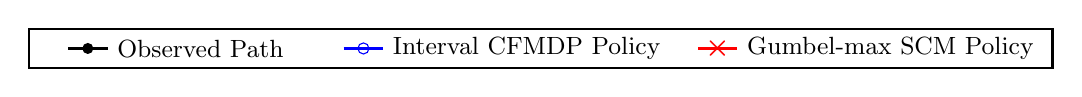
\begin{tikzpicture}[scale=1.0, every node/.style={scale=1.0}]
            \draw[thick, black] (-3, -0.25) rectangle (10, 0.25);
            %
            \draw[black, line width=1pt] (-2.5, 0.0) -- (-2,0.0);
            \fill[black] (-2.25,0.0) circle (2pt); %
            \node[right] at (-2,0.0) {\small Observed Path};
            
            %
            \draw[blue, line width=1pt] (1.0,0.0) -- (1.5,0.0);
            \node[draw=blue, circle, minimum size=4pt, inner sep=0pt] at (1.25,0.0) {}; %
            \node[right] at (1.5,0.0) {\small Interval CFMDP Policy};
            
            %
            \draw[red, line width=1pt] (5.5,0) -- (6,0);
            \node[red] at (5.75,0) {$\boldsymbol{\times}$}; %
            \node[right] at (6,0) {\small Gumbel-max SCM Policy};
        \end{tikzpicture}
    }\\
    %
    \subfigure[\footnotesize Lowest cumulative reward: Interval CFMDP ($312$), Gumbel-max SCM ($312$)]{%
        \resizebox{0.76\columnwidth}{!}{
             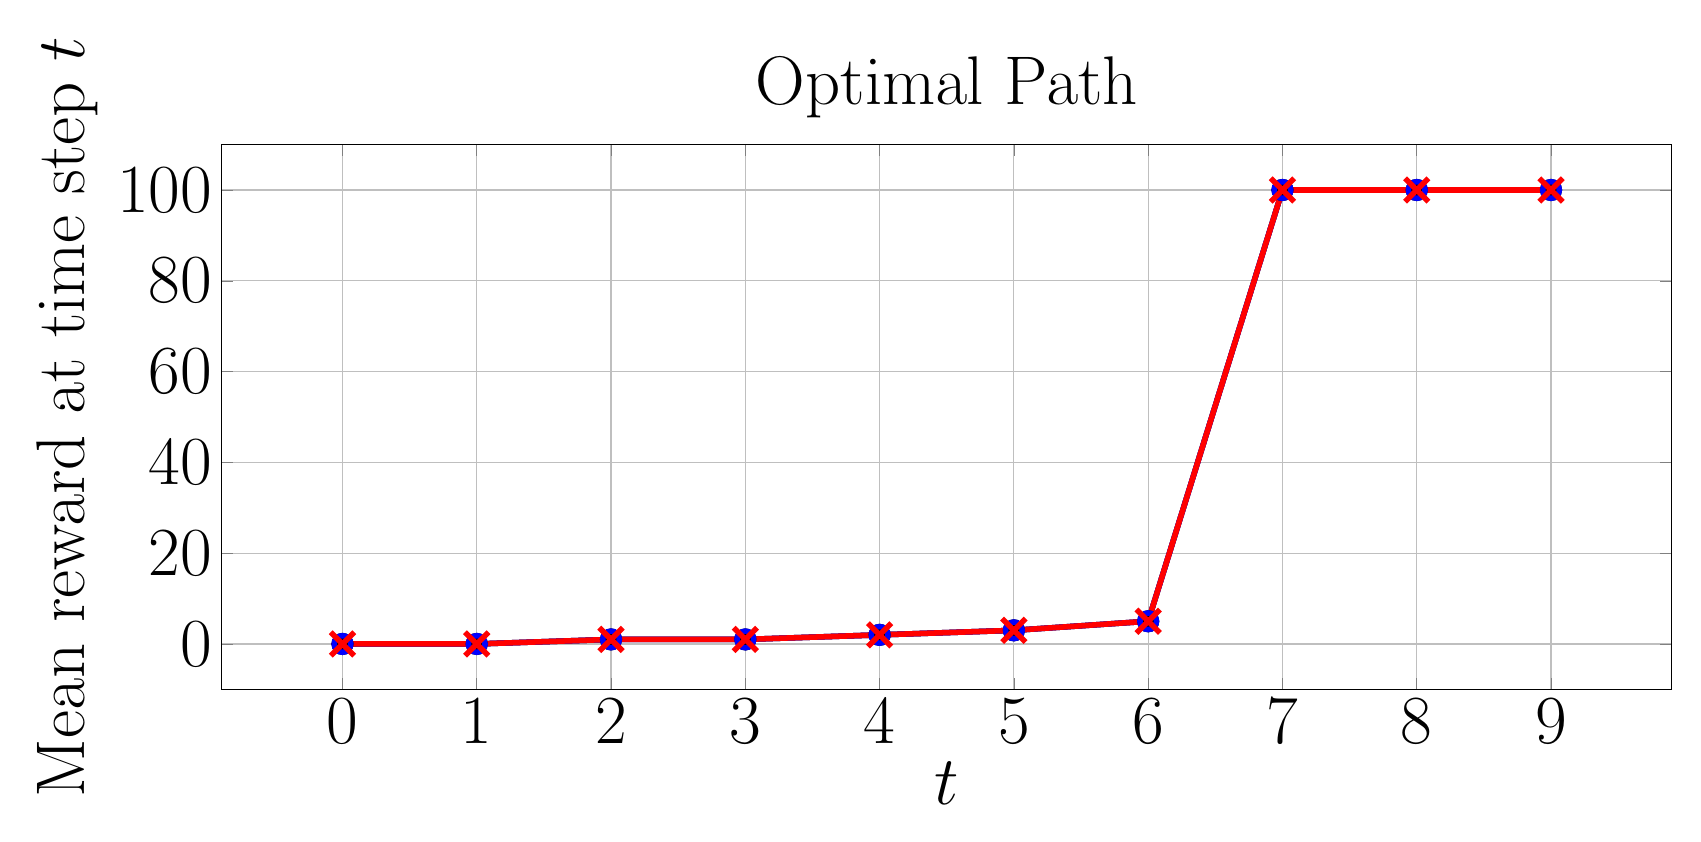
\begin{tikzpicture}
                \begin{axis}[
                    xlabel={$t$},
                    ylabel={Mean reward at time step $t$},
                    title={Optimal Path},
                    grid=both,
                    width=20cm, height=8.5cm,
                    every axis/.style={font=\Huge},
                    %
                ]
                \addplot[
                    color=black, %
                    mark=*, %
                    line width=2pt,
                    mark size=3pt,
                    error bars/.cd,
                    y dir=both, %
                    y explicit, %
                    error bar style={line width=1pt,solid},
                    error mark options={line width=1pt,mark size=4pt,rotate=90}
                ]
                coordinates {
                    (0, 0.0)  +- (0, 0.0)
                    (1, 0.0)  +- (0, 0.0) 
                    (2, 1.0)  +- (0, 0.0) 
                    (3, 1.0)  +- (0, 0.0)
                    (4, 2.0)  +- (0, 0.0)
                    (5, 3.0) +- (0, 0.0)
                    (6, 5.0) +- (0, 0.0)
                    (7, 100.0) +- (0, 0.0)
                    (8, 100.0) +- (0, 0.0)
                    (9, 100.0) +- (0, 0.0)
                };
                %
                \addplot[
                    color=blue, %
                    mark=o, %
                    line width=2pt,
                    mark size=3pt,
                    error bars/.cd,
                    y dir=both, %
                    y explicit, %
                    error bar style={line width=1pt,solid},
                    error mark options={line width=1pt,mark size=4pt,rotate=90}
                ]
                 coordinates {
                    (0, 0.0)  +- (0, 0.0)
                    (1, 0.0)  +- (0, 0.0) 
                    (2, 1.0)  +- (0, 0.0) 
                    (3, 1.0)  +- (0, 0.0)
                    (4, 2.0)  +- (0, 0.0)
                    (5, 3.0) +- (0, 0.0)
                    (6, 5.0) +- (0, 0.0)
                    (7, 100.0) +- (0, 0.0)
                    (8, 100.0) +- (0, 0.0)
                    (9, 100.0) +- (0, 0.0)
                };
                %
                \addplot[
                    color=red, %
                    mark=x, %
                    line width=2pt,
                    mark size=6pt,
                    error bars/.cd,
                    y dir=both, %
                    y explicit, %
                    error bar style={line width=1pt,solid},
                    error mark options={line width=1pt,mark size=4pt,rotate=90}
                ]
                coordinates {
                    (0, 0.0)  +- (0, 0.0)
                    (1, 0.0)  +- (0, 0.0) 
                    (2, 1.0)  +- (0, 0.0) 
                    (3, 1.0)  +- (0, 0.0)
                    (4, 2.0)  +- (0, 0.0)
                    (5, 3.0) +- (0, 0.0)
                    (6, 5.0) +- (0, 0.0)
                    (7, 100.0) +- (0, 0.0)
                    (8, 100.0) +- (0, 0.0)
                    (9, 100.0) +- (0, 0.0)
                };
                \end{axis}
            \end{tikzpicture}
         }
    }
    \hspace{1cm}
    \subfigure[\footnotesize Lowest cumulative reward: Interval CFMDP ($19$), Gumbel-max SCM ($-88$)]{%
         \resizebox{0.76\columnwidth}{!}{
            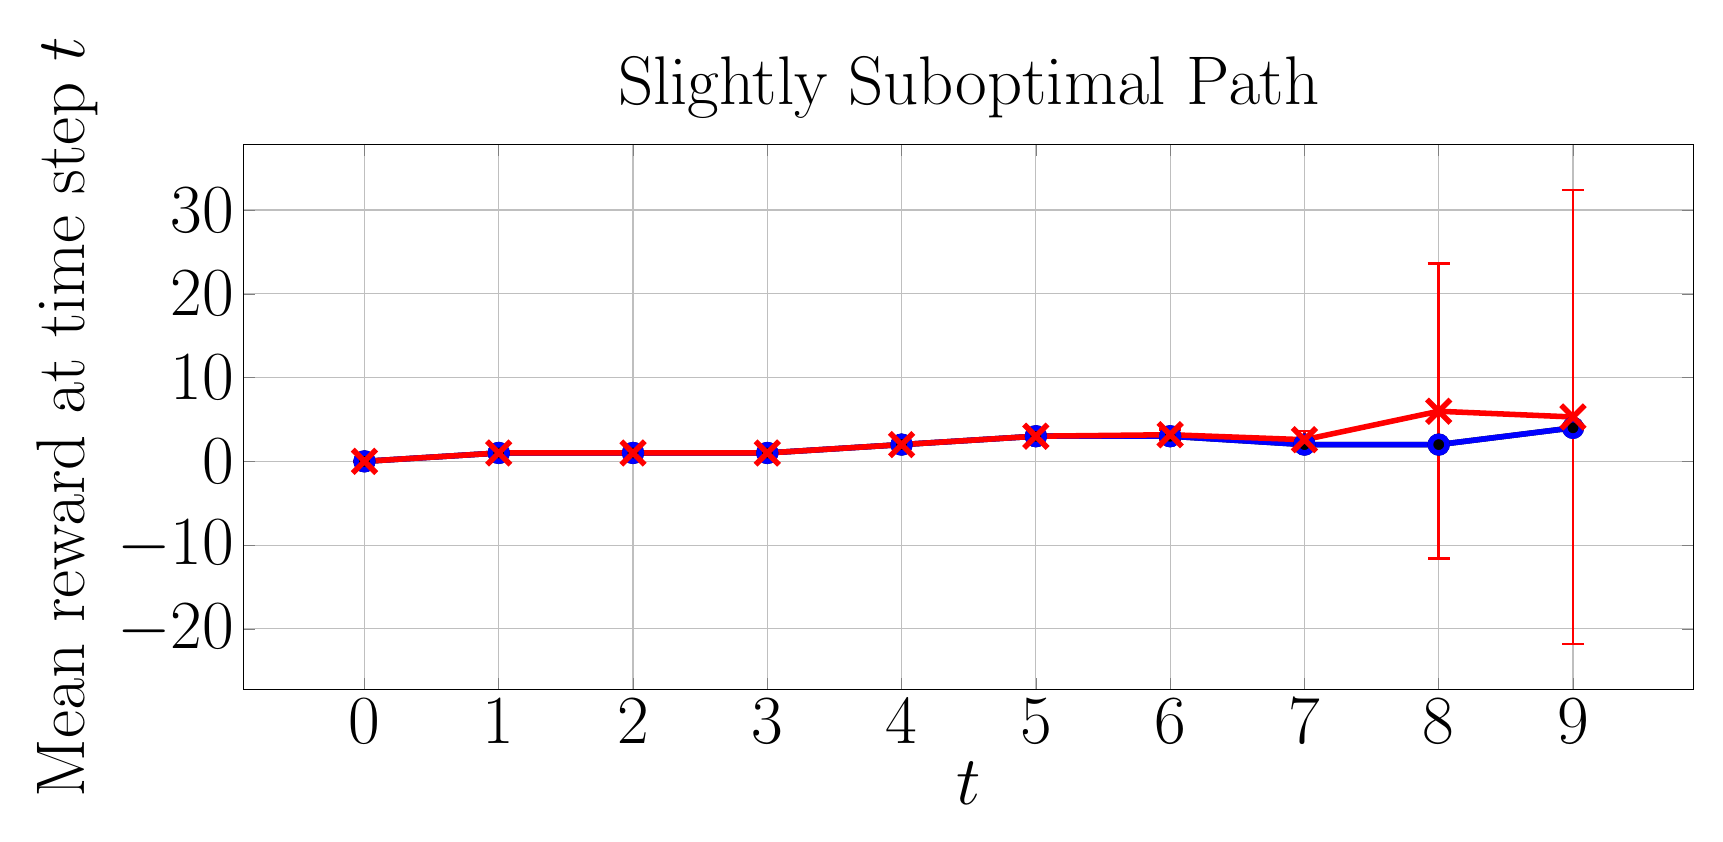
\begin{tikzpicture}
                \begin{axis}[
                    xlabel={$t$},
                    ylabel={Mean reward at time step $t$},
                    title={Slightly Suboptimal Path},
                    grid=both,
                    width=20cm, height=8.5cm,
                    every axis/.style={font=\Huge},
                    %
                ]
                \addplot[
                    color=black, %
                    mark=*, %
                    line width=2pt,
                    mark size=3pt,
                    error bars/.cd,
                    y dir=both, %
                    y explicit, %
                    error bar style={line width=1pt,solid},
                    error mark options={line width=1pt,mark size=4pt,rotate=90}
                ]
              coordinates {
                    (0, 0.0)  +- (0, 0.0)
                    (1, 1.0)  +- (0, 0.0) 
                    (2, 1.0)  +- (0, 0.0) 
                    (3, 1.0)  +- (0, 0.0)
                    (4, 2.0)  +- (0, 0.0)
                    (5, 3.0) +- (0, 0.0)
                    (6, 3.0) +- (0, 0.0)
                    (7, 2.0) +- (0, 0.0)
                    (8, 2.0) +- (0, 0.0)
                    (9, 4.0) +- (0, 0.0)
                };
                %
                \addplot[
                    color=blue, %
                    mark=o, %
                    line width=2pt,
                    mark size=3pt,
                    error bars/.cd,
                    y dir=both, %
                    y explicit, %
                    error bar style={line width=1pt,solid},
                    error mark options={line width=1pt,mark size=4pt,rotate=90}
                ]
              coordinates {
                    (0, 0.0)  +- (0, 0.0)
                    (1, 1.0)  +- (0, 0.0) 
                    (2, 1.0)  +- (0, 0.0) 
                    (3, 1.0)  +- (0, 0.0)
                    (4, 2.0)  +- (0, 0.0)
                    (5, 3.0) +- (0, 0.0)
                    (6, 3.0) +- (0, 0.0)
                    (7, 2.0) +- (0, 0.0)
                    (8, 2.0) +- (0, 0.0)
                    (9, 4.0) +- (0, 0.0)
                };
                %
                \addplot[
                    color=red, %
                    mark=x, %
                    line width=2pt,
                    mark size=6pt,
                    error bars/.cd,
                    y dir=both, %
                    y explicit, %
                    error bar style={line width=1pt,solid},
                    error mark options={line width=1pt,mark size=4pt,rotate=90}
                ]
                coordinates {
                    (0, 0.0)  +- (0, 0.0)
                    (1, 1.0)  +- (0, 0.0) 
                    (2, 1.0)  +- (0, 0.0) 
                    (3, 1.0)  +- (0, 0.0)
                    (4, 2.0)  += (0, 0.0)
                    (5, 3.0)  += (0, 0.0)
                    (6, 3.17847) += (0, 0.62606746) -= (0, 0.62606746)
                    (7, 2.5832885) += (0, 1.04598233) -= (0, 1.04598233)
                    (8, 5.978909) += (0, 17.60137623) -= (0, 17.60137623)
                    (9, 5.297059) += (0, 27.09227512) -= (0, 27.09227512)
                };
                \end{axis}
            \end{tikzpicture}
         }
    }\\[-1.5pt]
    \subfigure[\footnotesize Lowest cumulative reward: Interval CFMDP ($14$), Gumbel-max SCM ($-598$)]{%
         \resizebox{0.76\columnwidth}{!}{
             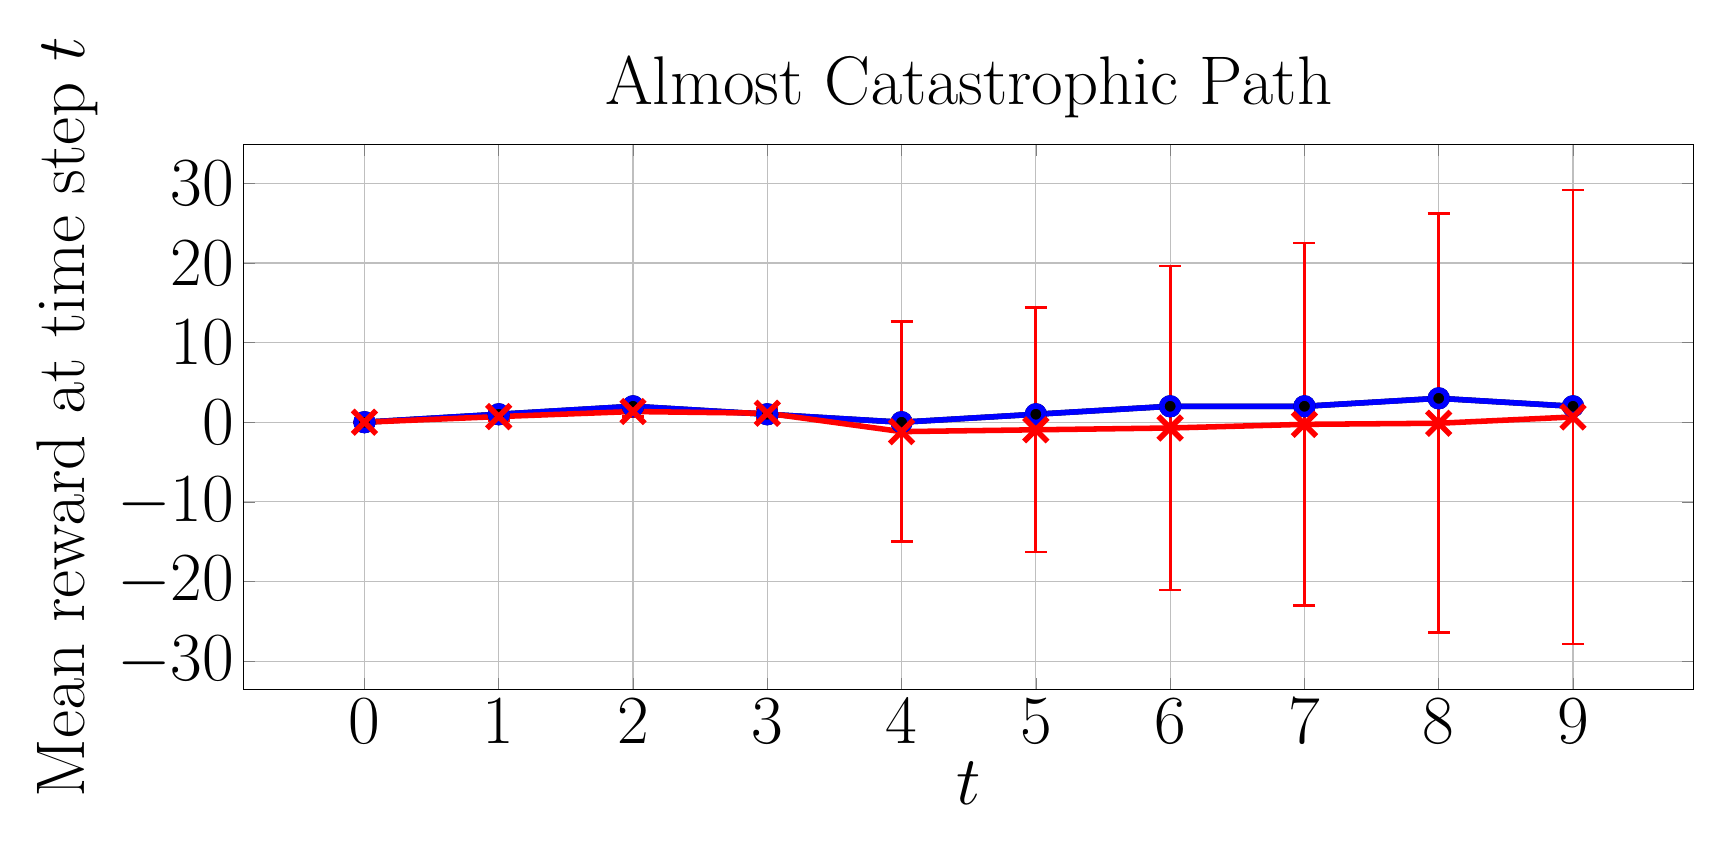
\begin{tikzpicture}
                \begin{axis}[
                    xlabel={$t$},
                    ylabel={Mean reward at time step $t$},
                    title={Almost Catastrophic Path},
                    grid=both,
                    width=20cm, height=8.5cm,
                    every axis/.style={font=\Huge},
                    %
                ]
                \addplot[
                    color=black, %
                    mark=*, %
                    line width=2pt,
                    mark size=3pt,
                    error bars/.cd,
                    y dir=both, %
                    y explicit, %
                    error bar style={line width=1pt,solid},
                    error mark options={line width=1pt,mark size=4pt,rotate=90}
                ]
                coordinates {
                    (0, 0.0)  +- (0, 0.0)
                    (1, 1.0)  +- (0, 0.0) 
                    (2, 2.0)  +- (0, 0.0) 
                    (3, 1.0)  +- (0, 0.0)
                    (4, 0.0)  +- (0, 0.0)
                    (5, 1.0) +- (0, 0.0)
                    (6, 2.0) +- (0, 0.0)
                    (7, 2.0) +- (0, 0.0)
                    (8, 3.0) +- (0, 0.0)
                    (9, 2.0) +- (0, 0.0)
                };
                %
                \addplot[
                    color=blue, %
                    mark=o, %
                    line width=2pt,
                    mark size=3pt,
                    error bars/.cd,
                    y dir=both, %
                    y explicit, %
                    error bar style={line width=1pt,solid},
                    error mark options={line width=1pt,mark size=4pt,rotate=90}
                ]
                coordinates {
                    (0, 0.0)  +- (0, 0.0)
                    (1, 1.0)  +- (0, 0.0) 
                    (2, 2.0)  +- (0, 0.0) 
                    (3, 1.0)  +- (0, 0.0)
                    (4, 0.0)  +- (0, 0.0)
                    (5, 1.0) +- (0, 0.0)
                    (6, 2.0) +- (0, 0.0)
                    (7, 2.0) +- (0, 0.0)
                    (8, 3.0) +- (0, 0.0)
                    (9, 2.0) +- (0, 0.0)
                };
                %
                \addplot[
                    color=red, %
                    mark=x, %
                    line width=2pt,
                    mark size=6pt,
                    error bars/.cd,
                    y dir=both, %
                    y explicit, %
                    error bar style={line width=1pt,solid},
                    error mark options={line width=1pt,mark size=4pt,rotate=90}
                ]
                coordinates {
                    (0, 0.0)  +- (0, 0.0)
                    (1, 0.7065655)  +- (0, 0.4553358) 
                    (2, 1.341673)  +- (0, 0.67091621) 
                    (3, 1.122926)  +- (0, 0.61281824)
                    (4, -1.1821935)  +- (0, 13.82444042)
                    (5, -0.952399)  +- (0, 15.35195457)
                    (6, -0.72672) +- (0, 20.33508414)
                    (7, -0.268983) +- (0, 22.77861454)
                    (8, -0.1310835) +- (0, 26.31013314)
                    (9, 0.65806) +- (0, 28.50670214)
                };
                %
            %
            %
            %
            %
            %
            %
            %
            %
            %
            %
            %
            %
            %
            %
            %
            %
            %
            %
                \end{axis}
            \end{tikzpicture}
         }
    }
    \hspace{1cm}
    \subfigure[\footnotesize Lowest cumulative reward: Interval CFMDP ($-698$), Gumbel-max SCM ($-698$)]{%
         \resizebox{0.76\columnwidth}{!}{
            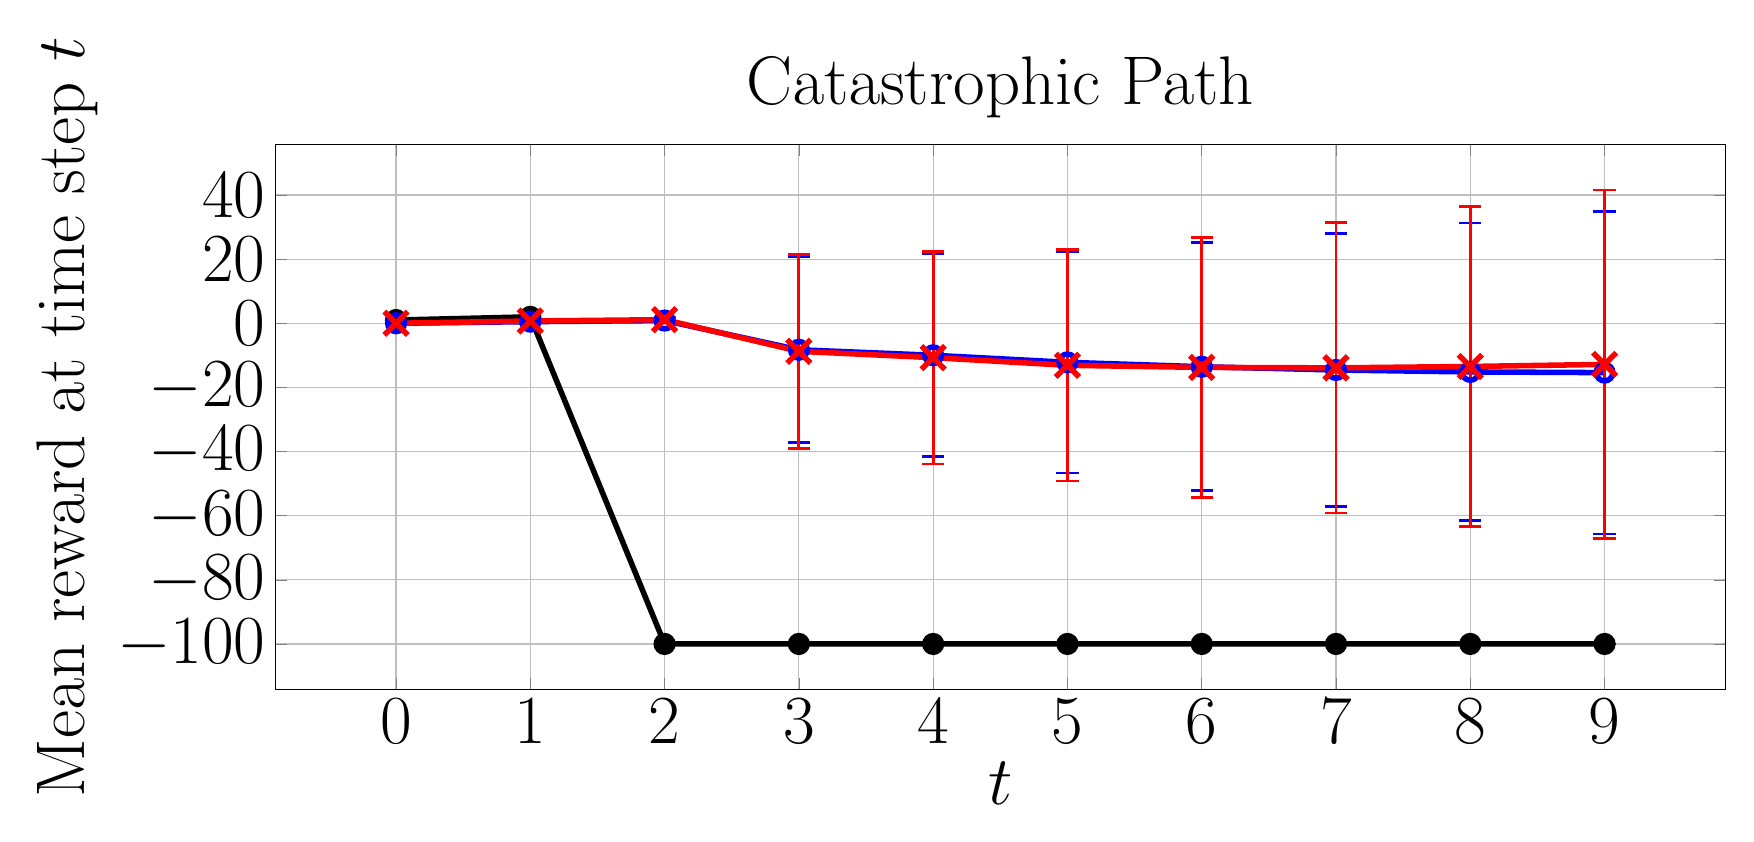
\begin{tikzpicture}
                \begin{axis}[
                    xlabel={$t$},
                    ylabel={Mean reward at time step $t$},
                    title={Catastrophic Path},
                    grid=both,
                    width=20cm, height=8.5cm,
                    every axis/.style={font=\Huge},
                    %
                ]
                \addplot[
                    color=black, %
                    mark=*, %
                    line width=2pt,
                    mark size=3pt,
                    error bars/.cd,
                    y dir=both, %
                    y explicit, %
                    error bar style={line width=1pt,solid},
                    error mark options={line width=1pt,mark size=4pt,rotate=90}
                ]
                coordinates {
                    (0, 1.0)  +- (0, 0.0)
                    (1, 2.0)  +- (0, 0.0) 
                    (2, -100.0)  +- (0, 0.0) 
                    (3, -100.0)  +- (0, 0.0)
                    (4, -100.0)  +- (0, 0.0)
                    (5, -100.0) +- (0, 0.0)
                    (6, -100.0) +- (0, 0.0)
                    (7, -100.0) +- (0, 0.0)
                    (8, -100.0) +- (0, 0.0)
                    (9, -100.0) +- (0, 0.0)
                };
                %
                \addplot[
                    color=blue, %
                    mark=o, %
                    line width=2pt,
                    mark size=3pt,
                    error bars/.cd,
                    y dir=both, %
                    y explicit, %
                    error bar style={line width=1pt,solid},
                    error mark options={line width=1pt,mark size=4pt,rotate=90}
                ]
                coordinates {
                    (0, 0.0)  +- (0, 0.0)
                    (1, 0.504814)  +- (0, 0.49997682) 
                    (2, 0.8439835)  +- (0, 0.76831917) 
                    (3, -8.2709165)  +- (0, 28.93656754)
                    (4, -9.981082)  +- (0, 31.66825363)
                    (5, -12.1776325) +- (0, 34.53463233)
                    (6, -13.556076) +- (0, 38.62845372)
                    (7, -14.574418) +- (0, 42.49603359)
                    (8, -15.1757075) +- (0, 46.41913968)
                    (9, -15.3900395) +- (0, 50.33563368)
                };
                %
                \addplot[
                    color=red, %
                    mark=x, %
                    line width=2pt,
                    mark size=6pt,
                    error bars/.cd,
                    y dir=both, %
                    y explicit, %
                    error bar style={line width=1pt,solid},
                    error mark options={line width=1pt,mark size=4pt,rotate=90}
                ]
                coordinates {
                    (0, 0.0)  +- (0, 0.0)
                    (1, 0.701873)  +- (0, 0.45743556) 
                    (2, 1.1227805)  +- (0, 0.73433129) 
                    (3, -8.7503255)  +- (0, 30.30257976)
                    (4, -10.722092)  +- (0, 33.17618589)
                    (5, -13.10721)  +- (0, 36.0648089)
                    (6, -13.7631645) +- (0, 40.56553451)
                    (7, -13.909043) +- (0, 45.23829402)
                    (8, -13.472517) +- (0, 49.96270296)
                    (9, -12.8278835) +- (0, 54.38618735)
                };
                %
            %
            %
            %
            %
            %
            %
            %
            %
            %
            %
            %
            %
            %
            %
            %
            %
            %
            %
                \end{axis}
            \end{tikzpicture}
         }
    }
    \caption{Average instant reward of CF paths induced by policies on GridWorld $p=0.4$.}
    \label{fig: reward p=0.4}
\end{figure*}

\subsection{Experimental Setup}
To compare policy performance, we measure the average rewards of counterfactual paths induced by our policy and the Gumbel-max policy by uniformly sampling $200$ counterfactual MDPs from the ICFMDP and generating $10,000$ counterfactual paths over each sampled CFMDP. \jl{Since the interval CFMDP depends on the observed path, we select $4$  paths of varying optimality to evaluate how the observed path impacts the performance of both policies: an optimal path, a slightly suboptimal path that could reach the optimal reward with a few changes, a catastrophic path that enters a catastrophic, terminal state with low reward, and an almost catastrophic path that was close to entering a catastrophic state.} When measuring the average probability bound widths and execution time needed to generate the ICFMDPs, we averaged over $20$ randomly generated observed paths
\footnote{Further training details are provided in Appendix \ref{app: training details}, and the code is provided at \href{https://github.com/ddv-lab/robust-cf-inference-in-MDPs}{https://github.com/ddv-lab/robust-cf-inference-in-MDPs}
%
%
.}.

\subsection{GridWorld}
\jl{The GridWorld MDP is a $4 \times 4$ grid where an agent must navigate from the top-left corner to the goal state in the bottom-right corner, avoiding a dangerous terminal state in the centre. At each time step, the agent can move up, down, left, or right, but there is a small probability (controlled by hyper-parameter $p$) of moving in an unintended direction. As the agent nears the goal, the reward for each state increases, culminating in a reward of $+100$ for reaching the goal. Entering the dangerous state results in a penalty of $-100$. We use two versions of GridWorld: a less stochastic version with $p=0.9$ (i.e., $90$\% chance of moving in the chosen direction) and a more stochastic version with $p=0.4$.}

\paragraph{GridWorld ($p=0.9$)}
When $p=0.9$, the counterfactual probability bounds are typically narrow (see Table \ref{tab:nonzero_probs} for average measurements). Consequently, as shown in Figure \ref{fig: reward p=0.9}, both policies are nearly identical and perform similarly well across the optimal, slightly suboptimal, and catastrophic paths.
%
However, for the almost catastrophic path, the interval CFMDP path is more conservative and follows the observed path more closely (as this is where the probability bounds are narrowest), which typically requires one additional step to reach the goal state than the Gumbel-max SCM policy.
%

\paragraph{GridWorld ($p=0.4$)}
\jl{When $p=0.4$, the GridWorld environment becomes more uncertain, increasing the risk of entering the dangerous state even if correct actions are chosen. Thus, as shown in Figure \ref{fig: reward p=0.4}, the interval CFMDP policy adopts a more conservative approach, avoiding deviation from the observed policy if it cannot guarantee higher counterfactual rewards (see the slightly suboptimal and almost catastrophic paths), whereas the Gumbel-max SCM is inconsistent: it can yield higher rewards, but also much lower rewards, reflected in the wide error bars.} For the catastrophic path, both policies must deviate from the observed path to achieve a higher reward and, in this case, perform similarly.
%
%
%
%
\subsection{Sepsis}
The Sepsis MDP \citep{oberst2019counterfactual} simulates trajectories of Sepsis patients. Each state consists of four vital signs (heart rate, blood pressure, oxygen concentration, and glucose levels), categorised as low, normal, or high.
and three treatments that can be toggled on/off at each time step (8 actions in total). Unlike \citet{oberst2019counterfactual}, we scale rewards based on the number of out-of-range vital signs, between $-1000$ (patient dies) and $1000$ (patient discharged). \jl{Like the GridWorld $p=0.4$ experiment, the Sepsis MDP is highly uncertain, as many states are equally likely to lead to optimal and poor outcomes. Thus, as shown in Figure \ref{fig: reward sepsis}, both policies follow the observed optimal and almost catastrophic paths to guarantee rewards are no worse than the observation.} However, improving the catastrophic path requires deviating from the observation. Here, the Gumbel-max SCM policy, on average, performs better than the interval CFMDP policy. But, since both policies have lower bounds clipped at $-1000$, neither policy reliably improves over the observation. In contrast, for the slightly suboptimal path, the interval CFMDP policy performs significantly better, shown by its higher lower bounds. 
Moreover, in these two cases, the worst-case counterfactual path generated by the interval CFMDP policy is better than that of the Gumbel-max SCM policy,
indicating its greater robustness.
%
\begin{figure*}
    \centering
     \resizebox{0.6\textwidth}{!}{
        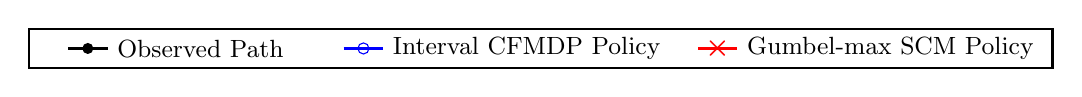
\begin{tikzpicture}[scale=1.0, every node/.style={scale=1.0}]
            \draw[thick, black] (-3, -0.25) rectangle (10, 0.25);
            %
            \draw[black, line width=1pt] (-2.5, 0.0) -- (-2,0.0);
            \fill[black] (-2.25,0.0) circle (2pt); %
            \node[right] at (-2,0.0) {\small Observed Path};
            
            %
            \draw[blue, line width=1pt] (1.0,0.0) -- (1.5,0.0);
            \node[draw=blue, circle, minimum size=4pt, inner sep=0pt] at (1.25,0.0) {}; %
            \node[right] at (1.5,0.0) {\small Interval CFMDP Policy};
            
            %
            \draw[red, line width=1pt] (5.5,0) -- (6,0);
            \node[red] at (5.75,0) {$\boldsymbol{\times}$}; %
            \node[right] at (6,0) {\small Gumbel-max SCM Policy};
        \end{tikzpicture}
    }\\
    \subfigure[\footnotesize Lowest cumulative reward: Interval CFMDP ($8000$), Gumbel-max SCM ($8000$)]{%
         \resizebox{0.76\columnwidth}{!}{
             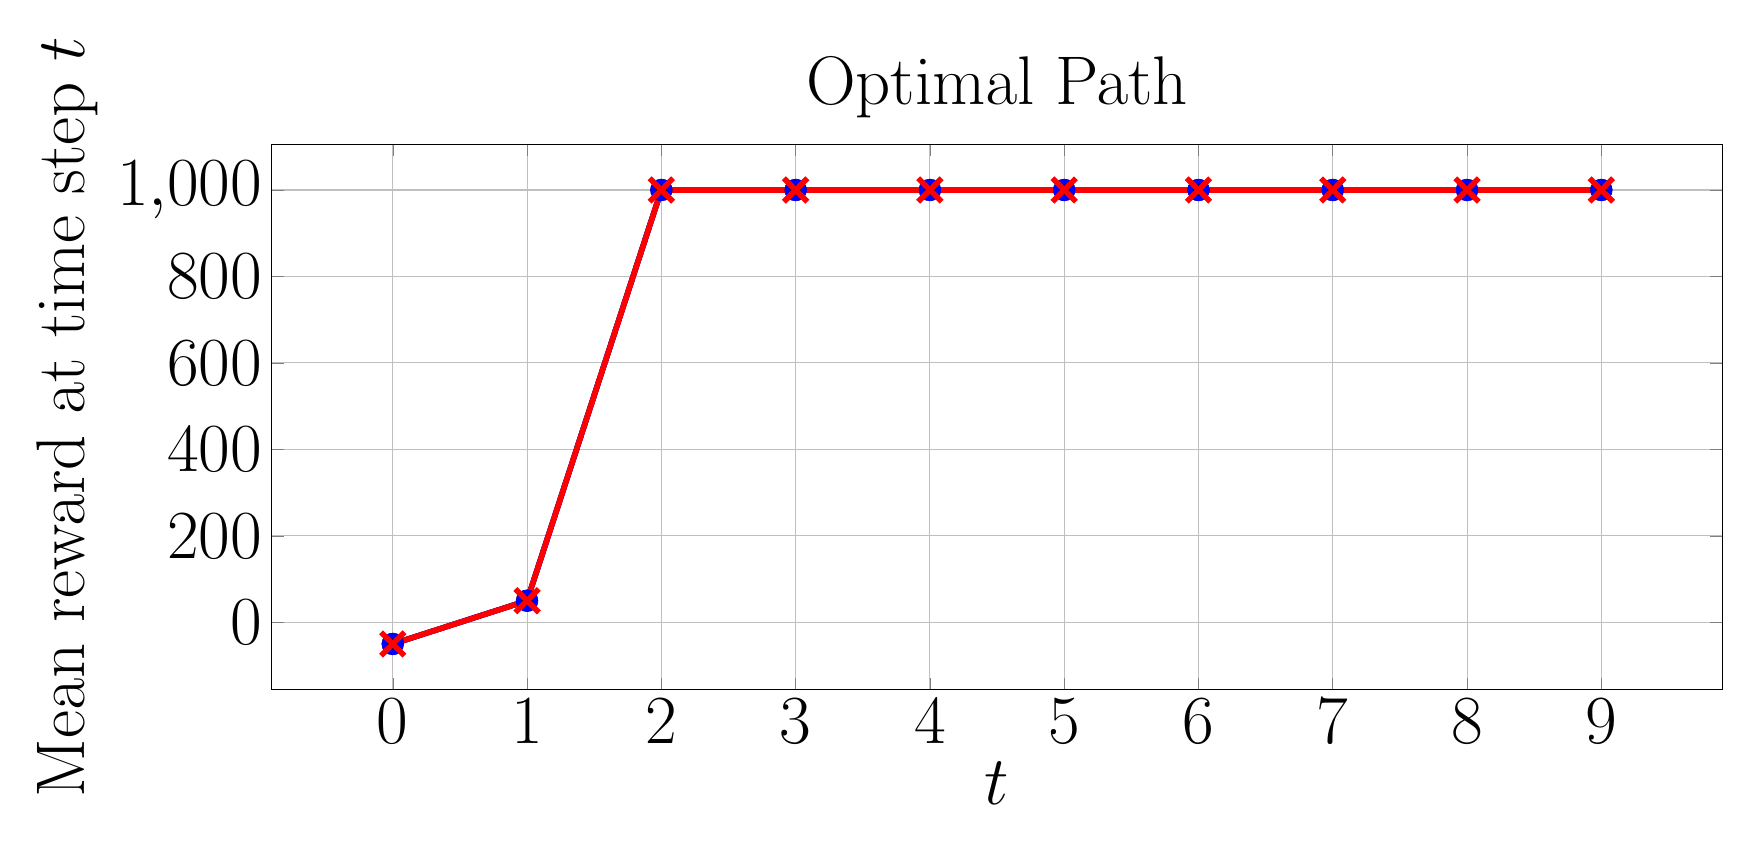
\begin{tikzpicture}
                \begin{axis}[
                    xlabel={$t$},
                    ylabel={Mean reward at time step $t$},
                    title={Optimal Path},
                    grid=both,
                    width=20cm, height=8.5cm,
                    every axis/.style={font=\Huge},
                    %
                ]
                \addplot[
                    color=black, %
                    mark=*, %
                    line width=2pt,
                    mark size=3pt,
                ]
                coordinates {
                    (0, -50.0)
                    (1, 50.0)
                    (2, 1000.0)
                    (3, 1000.0)
                    (4, 1000.0)
                    (5, 1000.0)
                    (6, 1000.0)
                    (7, 1000.0)
                    (8, 1000.0)
                    (9, 1000.0)
                };
                %
                \addplot[
                    color=blue, %
                    mark=o, %
                    line width=2pt,
                    mark size=3pt,
                    error bars/.cd,
                    y dir=both, %
                    y explicit, %
                    error bar style={line width=1pt,solid},
                    error mark options={line width=1pt,mark size=4pt,rotate=90}
                ]
                coordinates {
                    (0, -50.0)  +- (0, 0.0)
                    (1, 50.0)  +- (0, 0.0) 
                    (2, 1000.0)  +- (0, 0.0) 
                    (3, 1000.0)  +- (0, 0.0)
                    (4, 1000.0)  +- (0, 0.0)
                    (5, 1000.0) +- (0, 0.0)
                    (6, 1000.0) +- (0, 0.0)
                    (7, 1000.0) +- (0, 0.0)
                    (8, 1000.0) +- (0, 0.0)
                    (9, 1000.0) +- (0, 0.0)
                };
                %
                \addplot[
                    color=red, %
                    mark=x, %
                    line width=2pt,
                    mark size=6pt,
                    error bars/.cd,
                    y dir=both, %
                    y explicit, %
                    error bar style={line width=1pt,solid},
                    error mark options={line width=1pt,mark size=4pt,rotate=90}
                ]
                coordinates {
                    (0, -50.0)  +- (0, 0.0)
                    (1, 50.0)  +- (0, 0.0) 
                    (2, 1000.0)  +- (0, 0.0) 
                    (3, 1000.0)  +- (0, 0.0)
                    (4, 1000.0)  +- (0, 0.0)
                    (5, 1000.0) +- (0, 0.0)
                    (6, 1000.0) +- (0, 0.0)
                    (7, 1000.0) +- (0, 0.0)
                    (8, 1000.0) +- (0, 0.0)
                    (9, 1000.0) +- (0, 0.0)
                };
                %
                \end{axis}
            \end{tikzpicture}
         }
    }
    \hspace{1cm}
    \subfigure[\footnotesize Lowest cumulative reward: Interval CFMDP ($-5980$), Gumbel-max SCM ($-8000$)]{%
         \resizebox{0.76\columnwidth}{!}{
            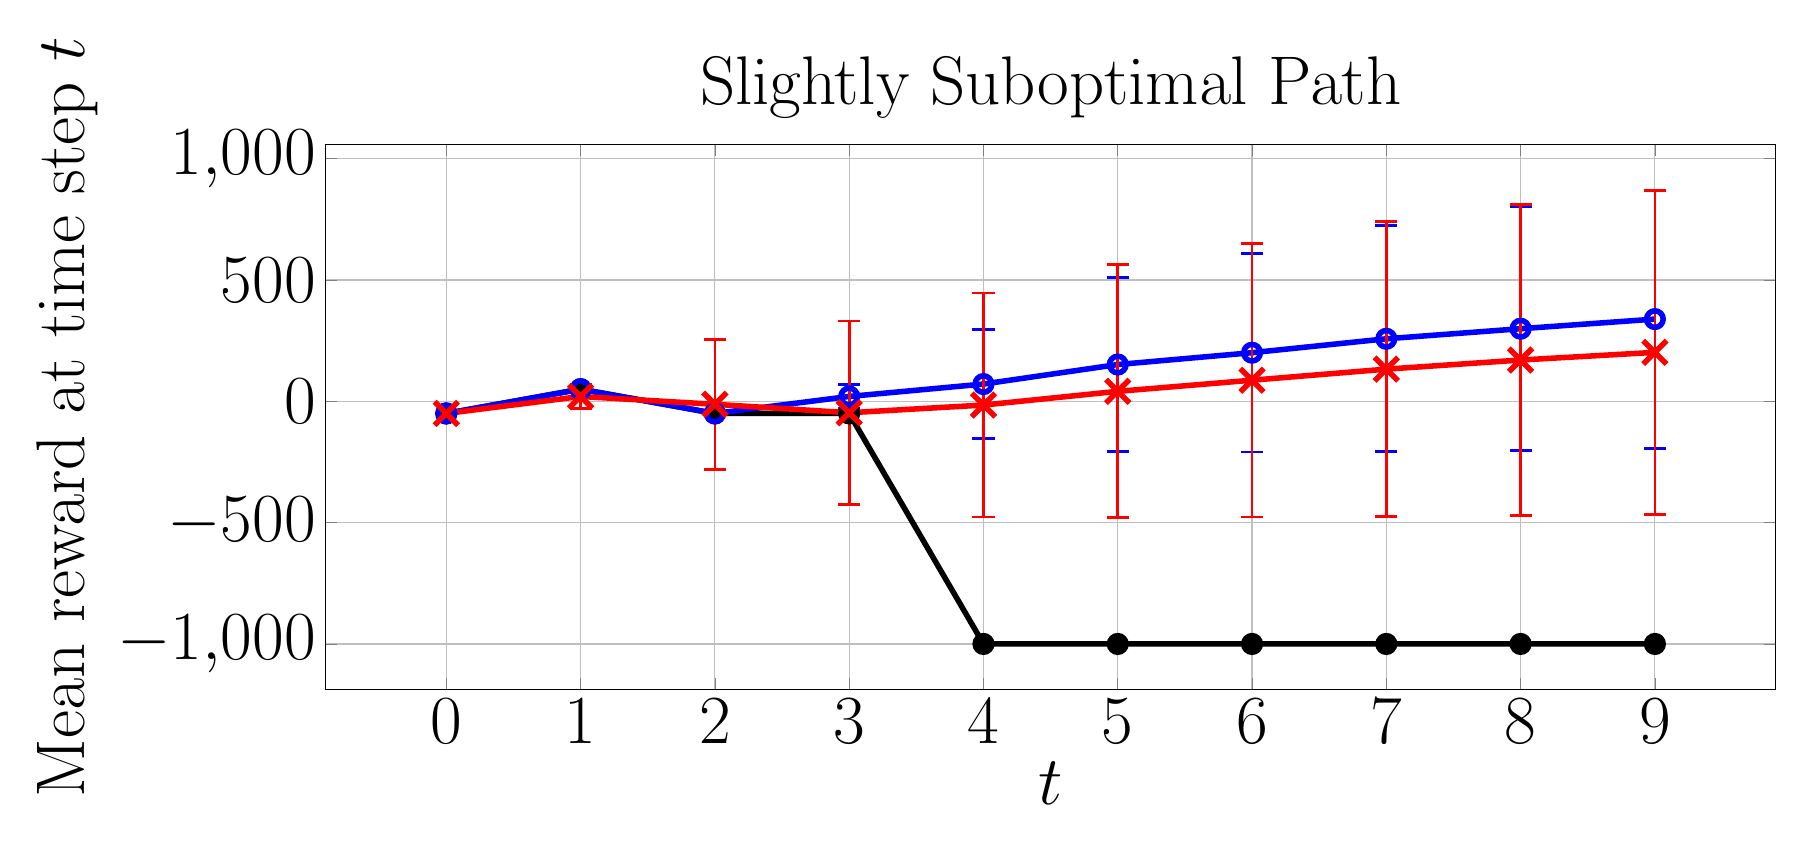
\begin{tikzpicture}
                \begin{axis}[
                    xlabel={$t$},
                    ylabel={Mean reward at time step $t$},
                    title={Slightly Suboptimal Path},
                    grid=both,
                    width=20cm, height=8.5cm,
                    every axis/.style={font=\Huge},
                    %
                ]
               \addplot[
                    color=black, %
                    mark=*, %
                    line width=2pt,
                    mark size=3pt,
                ]
                coordinates {
                    (0, -50.0)
                    (1, 50.0)
                    (2, -50.0)
                    (3, -50.0)
                    (4, -1000.0)
                    (5, -1000.0)
                    (6, -1000.0)
                    (7, -1000.0)
                    (8, -1000.0)
                    (9, -1000.0)
                };
                %
                \addplot[
                    color=blue, %
                    mark=o, %
                    line width=2pt,
                    mark size=3pt,
                    error bars/.cd,
                    y dir=both, %
                    y explicit, %
                    error bar style={line width=1pt,solid},
                    error mark options={line width=1pt,mark size=4pt,rotate=90}
                ]
                coordinates {
                    (0, -50.0)  +- (0, 0.0)
                    (1, 50.0)  +- (0, 0.0) 
                    (2, -50.0)  +- (0, 0.0) 
                    (3, 20.0631)  +- (0, 49.97539413)
                    (4, 71.206585)  +- (0, 226.02033693)
                    (5, 151.60797) +- (0, 359.23292559)
                    (6, 200.40593) +- (0, 408.86185176)
                    (7, 257.77948) +- (0, 466.10372804)
                    (8, 299.237465) +- (0, 501.82579506)
                    (9, 338.9129) +- (0, 532.06124996)
                };
                %
                \addplot[
                    color=red, %
                    mark=x, %
                    line width=2pt,
                    mark size=6pt,
                    error bars/.cd,
                    y dir=both, %
                    y explicit, %
                    error bar style={line width=1pt,solid},
                    error mark options={line width=1pt,mark size=4pt,rotate=90}
                ]
                coordinates {
                    (0, -50.0)  +- (0, 0.0)
                    (1, 20.00736)  +- (0, 49.99786741) 
                    (2, -12.282865)  +- (0, 267.598755) 
                    (3, -47.125995)  +- (0, 378.41755832)
                    (4, -15.381965)  +- (0, 461.77616558)
                    (5, 41.15459) +- (0, 521.53189262)
                    (6, 87.01595) +- (0, 564.22243126 )
                    (7, 132.62376) +- (0, 607.31338037)
                    (8, 170.168145) +- (0, 641.48013693)
                    (9, 201.813135) +- (0, 667.29441777)
                };
                %
                %
                %
                %
                %
                %
                %
                %
                %
                %
                %
                %
                %
                %
                %
                %
                %
                %
                %
                \end{axis}
            \end{tikzpicture}
         }
    }\\[-1.5pt]
    \subfigure[\footnotesize Lowest cumulative reward: Interval CFMDP ($100$), Gumbel-max SCM ($100$)]{%
         \resizebox{0.76\columnwidth}{!}{
             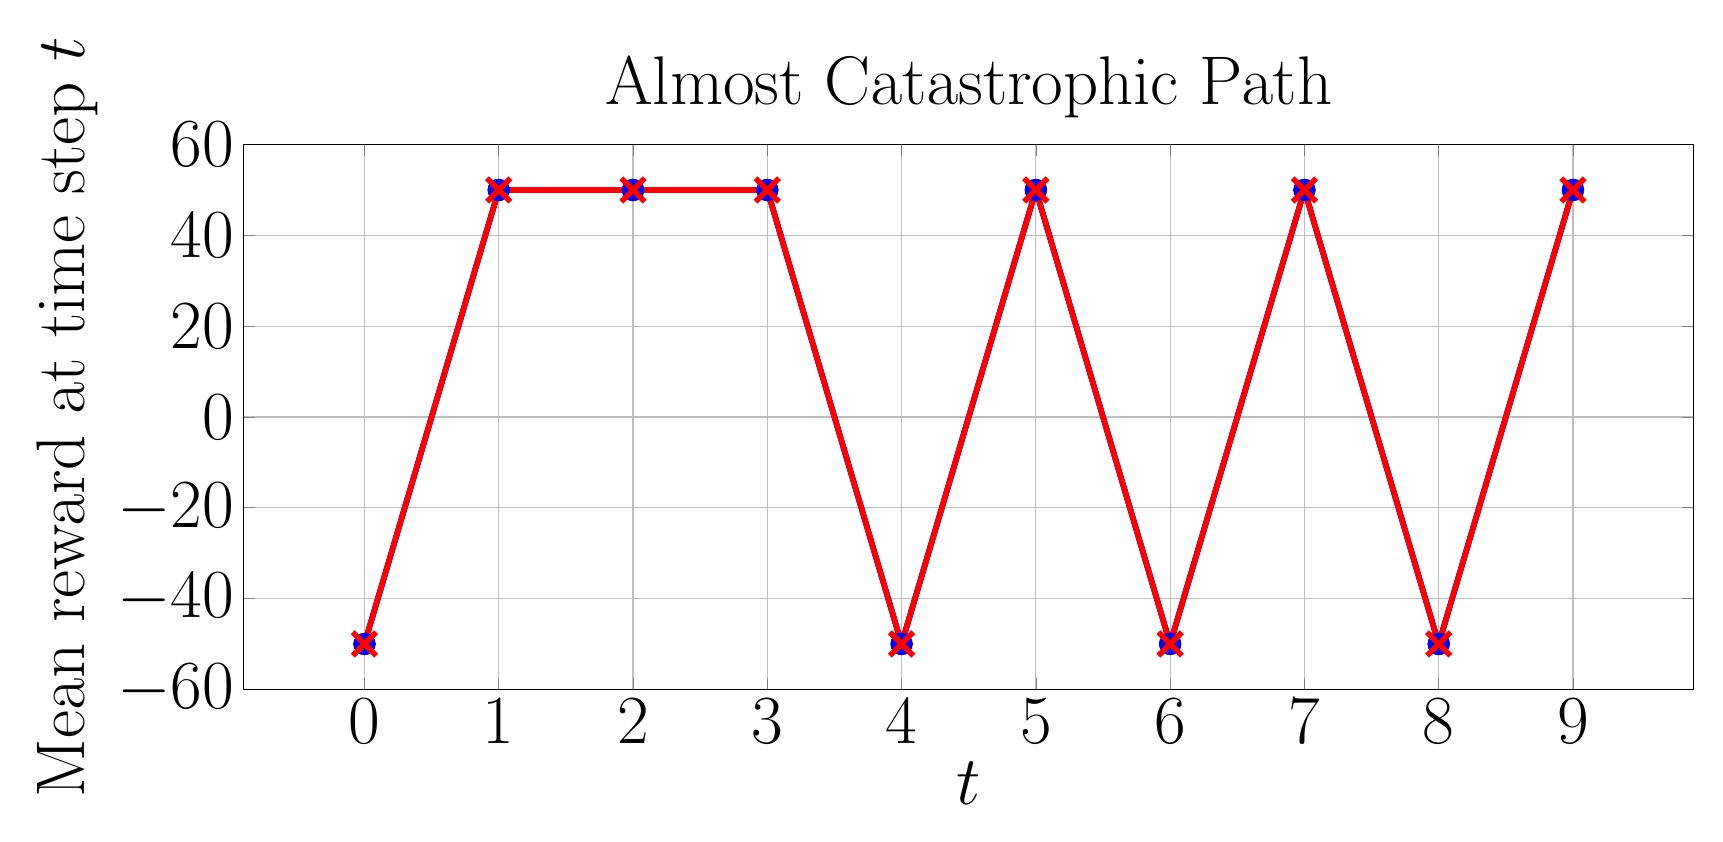
\begin{tikzpicture}
                \begin{axis}[
                    xlabel={$t$},
                    ylabel={Mean reward at time step $t$},
                    title={Almost Catastrophic Path},
                    grid=both,
                    every axis/.style={font=\Huge},
                    width=20cm, height=8.5cm,
                    %
                ]
               \addplot[
                    color=black, %
                    mark=*, %
                    line width=2pt,
                    mark size=3pt,
                ]
                coordinates {
                    (0, -50.0)
                    (1, 50.0)
                    (2, 50.0)
                    (3, 50.0)
                    (4, -50.0)
                    (5, 50.0)
                    (6, -50.0)
                    (7, 50.0)
                    (8, -50.0)
                    (9, 50.0)
                };
                %
                %
                \addplot[
                    color=blue, %
                    mark=o, %
                    line width=2pt,
                    mark size=3pt,
                    error bars/.cd,
                    y dir=both, %
                    y explicit, %
                    error bar style={line width=1pt,solid},
                    error mark options={line width=1pt,mark size=4pt,rotate=90}
                ]
                coordinates {
                    (0, -50.0)  +- (0, 0.0)
                    (1, 50.0)  +- (0, 0.0) 
                    (2, 50.0)  +- (0, 0.0) 
                    (3, 50.0)  +- (0, 0.0)
                    (4, -50.0)  +- (0, 0.0)
                    (5, 50.0) +- (0, 0.0)
                    (6, -50.0) +- (0, 0.0)
                    (7, 50.0) +- (0, 0.0)
                    (8, -50.0) +- (0, 0.0)
                    (9, 50.0) +- (0, 0.0)
                };
                %
                \addplot[
                    color=red, %
                    mark=x, %
                    line width=2pt,
                    mark size=6pt,
                    error bars/.cd,
                    y dir=both, %
                    y explicit, %
                    error bar style={line width=1pt,solid},
                    error mark options={line width=1pt,mark size=4pt,rotate=90}
                ]
                coordinates {
                    (0, -50.0)  +- (0, 0.0)
                    (1, 50.0)  +- (0, 0.0) 
                    (2, 50.0)  +- (0, 0.0) 
                    (3, 50.0)  +- (0, 0.0)
                    (4, -50.0)  +- (0, 0.0)
                    (5, 50.0) +- (0, 0.0)
                    (6, -50.0) +- (0, 0.0)
                    (7, 50.0) +- (0, 0.0)
                    (8, -50.0) +- (0, 0.0)
                    (9, 50.0) +- (0, 0.0)
                };
                %
                %
                %
                %
                %
                %
                %
                %
                %
                %
                %
                %
                %
                %
                %
                %
                %
                %
                %
                \end{axis}
            \end{tikzpicture}
         }
    }
    \hspace{1cm}
    \subfigure[\footnotesize Lowest cumulative reward: Interval CFMDP ($-7150$), Gumbel-max SCM ($-9050$)]{%
         \resizebox{0.76\columnwidth}{!}{
            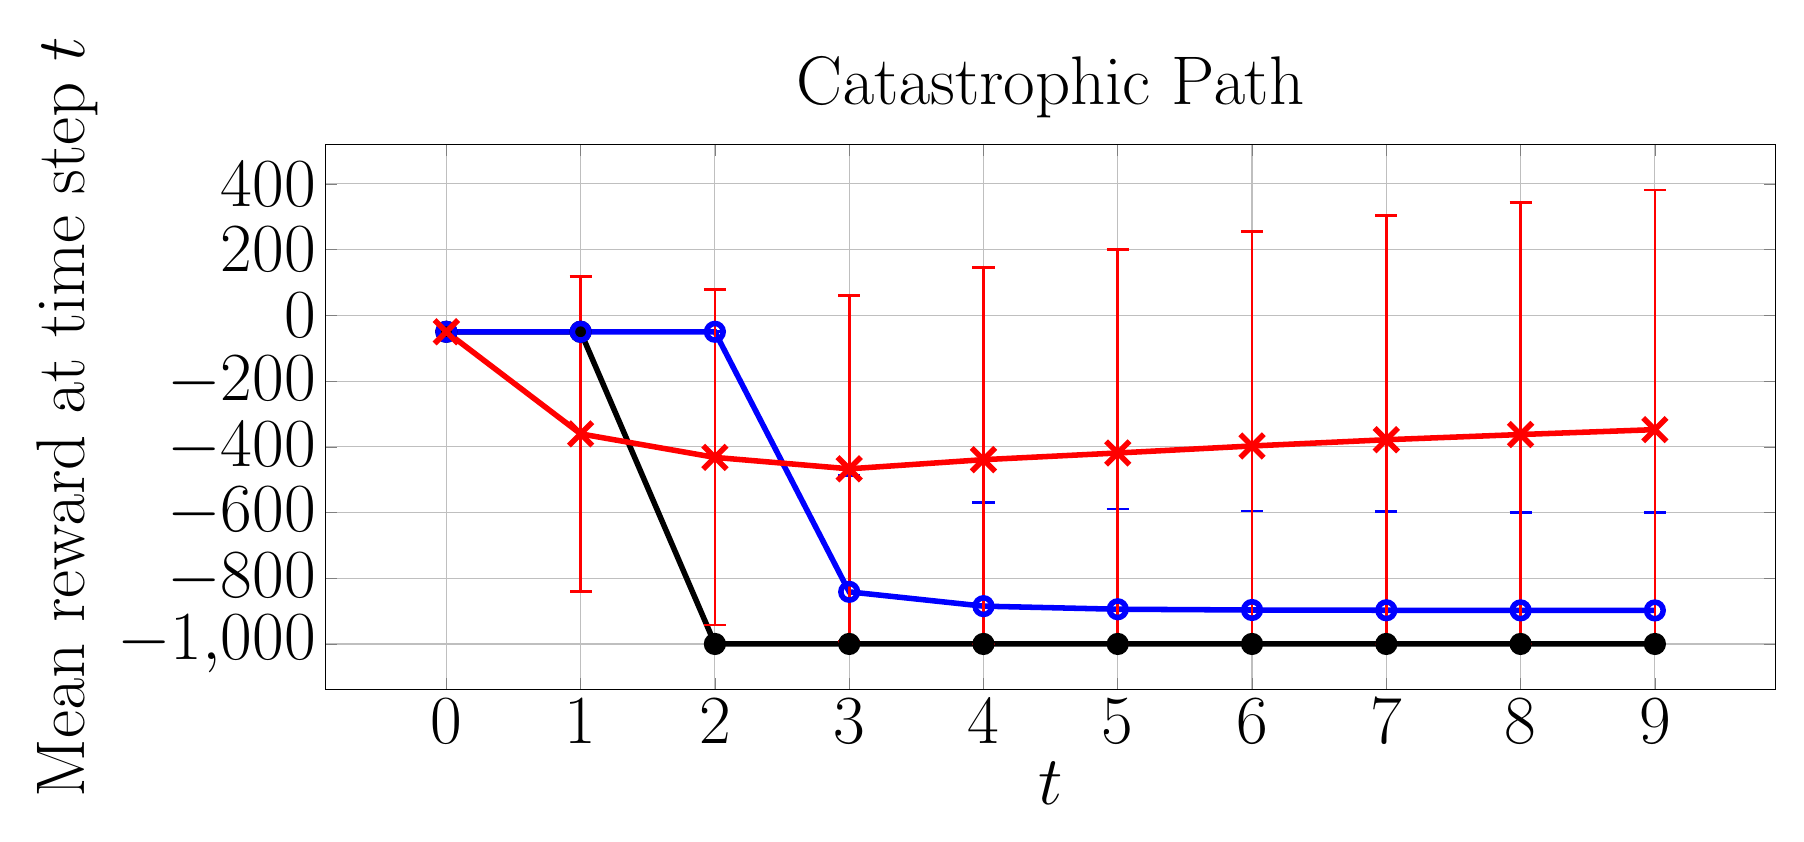
\begin{tikzpicture}
                \begin{axis}[
                    xlabel={$t$},
                    ylabel={Mean reward at time step $t$},
                    title={Catastrophic Path},
                    grid=both,
                    width=20cm, height=8.5cm,
                    every axis/.style={font=\Huge},
                    %
                ]
               \addplot[
                    color=black, %
                    mark=*, %
                    line width=2pt,
                    mark size=3pt,
                ]
                coordinates {
                    (0, -50.0)
                    (1, -50.0)
                    (2, -1000.0)
                    (3, -1000.0)
                    (4, -1000.0)
                    (5, -1000.0)
                    (6, -1000.0)
                    (7, -1000.0)
                    (8, -1000.0)
                    (9, -1000.0)
                };
                %
                %
                \addplot[
                    color=blue, %
                    mark=o, %
                    line width=2pt,
                    mark size=3pt,
                    error bars/.cd,
                    y dir=both, %
                    y explicit, %
                    error bar style={line width=1pt,solid},
                    error mark options={line width=1pt,mark size=4pt,rotate=90}
                ]
                coordinates {
                    (0, -50.0)  +- (0, 0.0)
                    (1, -50.0)  +- (0, 0.0) 
                    (2, -50.0)  +- (0, 0.0) 
                    (3, -841.440725)  += (0, 354.24605512) -= (0, 158.559275)
                    (4, -884.98225)  += (0, 315.37519669) -= (0, 115.01775)
                    (5, -894.330425) += (0, 304.88572805) -= (0, 105.669575)
                    (6, -896.696175) += (0, 301.19954514) -= (0, 103.303825)
                    (7, -897.4635) += (0, 299.61791279) -= (0, 102.5365)
                    (8, -897.77595) += (0, 298.80392585) -= (0, 102.22405)
                    (9, -897.942975) += (0, 298.32920557) -= (0, 102.057025)
                };
                %
                \addplot[
                    color=red, %
                    mark=x, %
                    line width=2pt,
                    mark size=6pt,
                    error bars/.cd,
                    y dir=both, %
                    y explicit, %
                    error bar style={line width=1pt,solid},
                    error mark options={line width=1pt,mark size=4pt,rotate=90}
                ]
            coordinates {
                    (0, -50.0)  +- (0, 0.0)
                    (1, -360.675265)  +- (0, 479.39812699) 
                    (2, -432.27629)  +- (0, 510.38620897) 
                    (3, -467.029545)  += (0, 526.36009628) -= (0, 526.36009628)
                    (4, -439.17429)  += (0, 583.96638919) -= (0, 560.82571)
                    (5, -418.82704) += (0, 618.43027478) -= (0, 581.17296)
                    (6, -397.464895) += (0, 652.67322574) -= (0, 602.535105)
                    (7, -378.49052) += (0, 682.85407033) -= (0, 621.50948)
                    (8, -362.654195) += (0, 707.01412023) -= (0, 637.345805)
                    (9, -347.737935) += (0, 729.29076479) -= (0, 652.262065)
                };
                %
                %
                %
                %
                %
                %
                %
                %
                %
                %
                %
                %
                %
                %
                %
                %
                %
                %
                %
                \end{axis}
            \end{tikzpicture}
         }
    }
    \caption{Average instant reward of CF paths induced by policies on Sepsis.}
    \label{fig: reward sepsis}
\end{figure*}

%
%
%
\subsection{Interval CFMDP Bounds}
%
%
Table \ref{tab:nonzero_probs} presents the mean counterfactual probability bound widths (excluding transitions where the upper bound is $0$) for each MDP, averaged over 20 observed paths. We compare the bounds under counterfactual stability (CS) and monotonicity (M) assumptions, CS alone, and no assumptions. This shows that the assumptions marginally reduce the bound widths, indicating the assumptions tighten the bounds without excluding too many causal models, as intended.
\renewcommand{\arraystretch}{1}

\begin{table}
\centering
\caption{Mean width of counterfactual probability bounds}
\resizebox{0.8\columnwidth}{!}{%
\begin{tabular}{|c|c|c|c|}
\hline
\multirow{2}{*}{\textbf{Environment}} & \multicolumn{3}{c|}{\textbf{Assumptions}} \\ \cline{2-4}
 & \textbf{CS + M} & \textbf{CS} & \textbf{None\tablefootnote{\jl{Equivalent to \citet{li2024probabilities}'s bounds (see Section \ref{sec: equivalence with Li}).}}} \\ \hline
\textbf{GridWorld} ($p=0.9$) & 0.0817 & 0.0977 & 0.100 \\ \hline
\textbf{GridWorld} ($p=0.4$) & 0.552  & 0.638  & 0.646 \\ \hline
\textbf{Sepsis} & 0.138 & 0.140 & 0.140 \\ \hline
\end{tabular}
}
\label{tab:nonzero_probs}
\end{table}


\subsection{Execution Times}
Table \ref{tab: times} compares the average time needed to generate the interval CFMDP vs.\ the Gumbel-max SCM CFMDP for 20 observations.
The GridWorld algorithms were run single-threaded, while the Sepsis experiments were run in parallel.
Generating the interval CFMDP is significantly faster as it uses exact analytical bounds, whereas the Gumbel-max CFMDP requires sampling from the Gumbel distribution to estimate counterfactual transition probabilities. \jl{Since constructing the counterfactual MDP models is the main bottleneck in both approaches, ours is more efficient overall and suitable for larger MDPs.}
\begin{table}
\centering
\caption{Mean execution time to generate CFMDPs}
\resizebox{0.99\columnwidth}{!}{%
\begin{tabular}{|c|c|c|}
\hline
\multirow{2}{*}{\textbf{Environment}} & \multicolumn{2}{c|}{\textbf{Mean Execution Time (s)}} \\ \cline{2-3} 
                                      & \textbf{Interval CFMDP} & \textbf{Gumbel-max CFMDP} \\ \hline
\textbf{GridWorld ($p=0.9$) }                  & 0.261                   & 56.1                      \\ \hline
\textbf{GridWorld ($p=0.4$)  }                 & 0.336                   & 54.5                      \\ \hline
\textbf{Sepsis}                                 & 688                     & 2940                      \\ \hline
\end{tabular}%
}
\label{tab: times}
\end{table}


% \section{Threads to Validity}
% \label{sec:validity}
% \section{Research Trustworthiness, Limitations and Trade-offs}\label{sec:trust}

\subsection{Trustworthiness}

\noindent We implemented several techniques to address the requirements of research trustworthiness \citep{miles2014qualitative}. We reported \textit{Saturation} (Phase I), \textit{Member checking} (Phase I), and \emph{Feedback session} (Phase II) in Sect. \ref{sec:methods}.

\textit{Triangulation}: We triangulated data sources, including interviews, focus groups, and participant feedback sessions. This exercise allowed us to ensure that our findings are corroborated across different data sources and contexts.

\textit{Peer debriefing}: Although the analysis was primarily conducted by the first author, the second and third authors reviewed the proposed codes, and the results were continuously discussed and scrutinized by the other two authors in several meetings throughout the analysis process. The participation of two authors in the coding process helped minimize researcher biases \citep{miles2014qualitative}. This approach is grounded in our epistemological stance, constructivism, which posits that knowledge is socially constructed and that collective intellectual engagement can lead to more reliable understandings of the data \citep{fosnot2013constructivism}. 

\textit{Thick description}: We endeavored to provide a detailed explanation of our research process and the decisions we have made throughout (see Sect. \ref{sec:methods}). In addition, we assembled a comprehensive replication package (see Sect. \ref{sec:replication}).

\subsection{Limitations and Trade-offs}\label{sec:limit}

\textit{Homogeneous sample}: Our sample is composed only of software engineers. In line with roles theory \citep{katz1978social,frink2004advancing}, we limited our sample to the software engineer role to mitigate the potential for variations that may arise by the inclusion of multiple roles. Roles theory suggests that individuals' accountability is closely linked to roles \citep{katz1978social,frink2004advancing}. This narrow focus strengthens the internal validity of our study and allows for role-centric conclusions.

\textit{Focus on intrinsic drivers}: By focusing primarily on intrinsic drivers and their influence on accountability, we may have inadvertently undermined other factors. For example, in our previous work, we identified institutional factors, such as financial incentives or denial of promotions, that also promote accountability in SE environments \citep{alami2024understanding}. 

\textit{Limited variation in the focus group design}: Another tradeoff is the limited number of variations in the focus group configurations, and the code snippets we used were not of industrial caliber. The consistency across the four groups, shown in the collected data and findings, suggests that additional configurations might not have significantly altered the results. In addition, we prioritized in-depth discussions, which may have been diluted by overly complicated configurations and complex code.

Another tradeoff for this study design is with more realistic, complex, and context-aware code. However, we felt this would greatly limit the accessibility of the focus groups. A future study, examining the contextual intricacies of a proprietary codebase, would shed insight on the role of context in this setting.

We conducted focus groups synchronously and online. Often code reviews, in particular on GitHub and similar sites, are asynchronous and text-based. Open source projects have different dynamics than the ones we discuss here. Hence, our findings our findings may not fully transferable to asynchronous or open-source code reviews. Furthermore, the online setting may have influenced participants' behavior differently than an in-person setup. 

The implementation of a pre-focus group questionnaire to mitigate the risk of social desirability bias \citep{furnham1986response} and self-censorship \citep{yanos2008false} during the focus group discussions carries the risk of priming participants. To mitigate this risk, we avoided the explicit use of the word ``accountability'' in the questions. In addition, during the discussions, we asked participants to provide concrete examples to anchor their responses in their personal experiences, thereby avoiding generic or socially desired answers.



\section{Related Work}
\label{sec:related}
\putsec{related}{Related Work}

\noindent \textbf{Efficient Radiance Field Rendering.}
%
The introduction of Neural Radiance Fields (NeRF)~\cite{mil:sri20} has
generated significant interest in efficient 3D scene representation and
rendering for radiance fields.
%
Over the past years, there has been a large amount of research aimed at
accelerating NeRFs through algorithmic or software
optimizations~\cite{mul:eva22,fri:yu22,che:fun23,sun:sun22}, and the
development of hardware
accelerators~\cite{lee:cho23,li:li23,son:wen23,mub:kan23,fen:liu24}.
%
The state-of-the-art method, 3D Gaussian splatting~\cite{ker:kop23}, has
further fueled interest in accelerating radiance field
rendering~\cite{rad:ste24,lee:lee24,nie:stu24,lee:rho24,ham:mel24} as it
employs rasterization primitives that can be rendered much faster than NeRFs.
%
However, previous research focused on software graphics rendering on
programmable cores or building dedicated hardware accelerators. In contrast,
\name{} investigates the potential of efficient radiance field rendering while
utilizing fixed-function units in graphics hardware.
%
To our knowledge, this is the first work that assesses the performance
implications of rendering Gaussian-based radiance fields on the hardware
graphics pipeline with software and hardware optimizations.

%%%%%%%%%%%%%%%%%%%%%%%%%%%%%%%%%%%%%%%%%%%%%%%%%%%%%%%%%%%%%%%%%%%%%%%%%%
\myparagraph{Enhancing Graphics Rendering Hardware.}
%
The performance advantage of executing graphics rendering on either
programmable shader cores or fixed-function units varies depending on the
rendering methods and hardware designs.
%
Previous studies have explored the performance implication of graphics hardware
design by developing simulation infrastructures for graphics
workloads~\cite{bar:gon06,gub:aam19,tin:sax23,arn:par13}.
%
Additionally, several studies have aimed to improve the performance of
special-purpose hardware such as ray tracing units in graphics
hardware~\cite{cho:now23,liu:cha21} and proposed hardware accelerators for
graphics applications~\cite{lu:hua17,ram:gri09}.
%
In contrast to these works, which primarily evaluate traditional graphics
workloads, our work focuses on improving the performance of volume rendering
workloads, such as Gaussian splatting, which require blending a huge number of
fragments per pixel.

%%%%%%%%%%%%%%%%%%%%%%%%%%%%%%%%%%%%%%%%%%%%%%%%%%%%%%%%%%%%%%%%%%%%%%%%%%
%
In the context of multi-sample anti-aliasing, prior work proposed reducing the
amount of redundant shading by merging fragments from adjacent triangles in a
mesh at the quad granularity~\cite{fat:bou10}.
%
While both our work and quad-fragment merging (QFM)~\cite{fat:bou10} aim to
reduce operations by merging quads, our proposed technique differs from QFM in
many aspects.
%
Our method aims to blend \emph{overlapping primitives} along the depth
direction and applies to quads from any primitive. In contrast, QFM merges quad
fragments from small (e.g., pixel-sized) triangles that \emph{share} an edge
(i.e., \emph{connected}, \emph{non-overlapping} triangles).
%
As such, QFM is not applicable to the scenes consisting of a number of
unconnected transparent triangles, such as those in 3D Gaussian splatting.
%
In addition, our method computes the \emph{exact} color for each pixel by
offloading blending operations from ROPs to shader units, whereas QFM
\emph{approximates} pixel colors by using the color from one triangle when
multiple triangles are merged into a single quad.



\section{Conclusion and Future Work}
\label{sec:conclusion}
\section{Conclusion}
In this work, we propose a simple yet effective approach, called SMILE, for graph few-shot learning with fewer tasks. Specifically, we introduce a novel dual-level mixup strategy, including within-task and across-task mixup, for enriching the diversity of nodes within each task and the diversity of tasks. Also, we incorporate the degree-based prior information to learn expressive node embeddings. Theoretically, we prove that SMILE effectively enhances the model's generalization performance. Empirically, we conduct extensive experiments on multiple benchmarks and the results suggest that SMILE significantly outperforms other baselines, including both in-domain and cross-domain few-shot settings.



% conference papers do not normally have an appendix


% use section* for acknowledgment
% \section*{Acknowledgment}


% The authors would like to thank...
\bibliographystyle{IEEEtranN}
\bibliography{sample}

% \vskip -2.5\baselineskip plus -1fil
\begin{IEEEbiographynophoto}{Krithika Iyer} is a computing PhD candidate at the Kahlert School of Computing and 
the Scientific Computing and Imaging Institute at the University of Utah in the Image Analysis track. She received her B.E. in Electronics \& Telecommunication in 2015. Her research interests include medical image analysis, probabilistic modeling, deep learning, and statistical shape modeling.\end{IEEEbiographynophoto}
\vskip -2.5\baselineskip plus -1fil
\begin{IEEEbiographynophoto}{Mokshagna Sai Teja Karanam} is a computing PhD student at the Kahlert School of Computing and the Scientific Computing and Imaging Institute at the University of Utah in the Image Analysis track. He received his B.E. in Computer Science in 2020 and his Masters in 2024. His research interests include deep learning, computer vision and statistical shape modeling.\end{IEEEbiographynophoto}
\vskip -2.5\baselineskip plus -1fil
\begin{IEEEbiographynophoto}{Shireen Elhabian} is a faculty member at the Kahlert School of Computing and the Scientific Computing and Imaging Institute at the University of Utah. Her research focuses on enhancing diagnostic accuracy through deep learning, probabilistic modeling, and advanced computer vision algorithms. She has published over 100 peer-reviewed publications in prestigious journals and conferences, including IEEE-TMI, MedIA, ICLR, CVPR, ICCV, MICCAI, IPMI, AAAI. \end{IEEEbiographynophoto}
\vskip -3\baselineskip plus -1fil



% that's all folks
\end{document}

